%!TEX encoding = UTF-8 Unicode
%!TEX TS-program = pdflatex

%%% --- PREAMBLE --- %%%

\documentclass[a4paper,11pt]{article}

\usepackage[italian]{babel}
\usepackage[left=2cm,right=2cm,top=2cm,bottom=2cm]{geometry}
\usepackage[T1]{fontenc} % OT1: basic, T1: western, T3 and T5: exotic, T4: lots of characters but WORSE READABILITY
\usepackage[utf8x]{inputenc} % utf8x supports more characters than utf8
\usepackage{graphicx} % import PNG, JPG and PDF with \includegraphics
\usepackage[usenames,table]{xcolor} % \color
\usepackage{amssymb}
\usepackage{amsmath}
\usepackage{amsfonts}
\usepackage{mathtools} % (!! PLACE BEFORE hyperref !!)
\usepackage{xfrac} % \sfrac
\usepackage{cancel} % \cancel \cancelto
\usepackage{hyperref} % interactive links in TOC, URLs and references
% unneded \usepackage{fixltx2e} % provides \textsubscript and makes some fixes
\usepackage[version=3]{mhchem} % \ce (chemical formula)
\usepackage{siunitx} % \num \si \SI
\usepackage{alltt} % {alltt} (like verbatim but with commands)
\usepackage{moreverb} % {listing}
\usepackage{listings} % {lstlisting}
\usepackage[overload]{textcase} % fixes \MakeUppercase and \MakeLowercase
\usepackage[normalem]{ulem} % \uline \uwave \sout \xout
\usepackage{enumerate} % adds options for {enumerate}
\usepackage{paralist} % inline lists with {inparaenum}
\usepackage[official]{eurosym} % \euro
\usepackage{tabu} % {tabu} (like {tabular} with improvements)
\usepackage{layout} % layout description
\usepackage{multicol} % {multicols}
\usepackage{lipsum} % filling text generator with \lipsum
\usepackage[section]{placeins} % inhibits float figures from trepassing a section boundary
\usepackage{subfig} % \subfloat to be used inside {figure}
\usepackage{wrapfig} % {wrapfigure} (like {figure} but allows text to flow on its sides)
\usepackage{ifthen} % \ifthenelse
\usepackage{calc}
\usepackage{array}
\usepackage{multirow}
\usepackage{booktabs} % \toprule, \midrule, \bottomrule
\graphicspath{ {../Figs-Tabs/} } % graphics search directories
\setcounter{tocdepth}{1} % -1: part, 0: chapter, 1: section, 2: subsection, 3: subsubsection

\lstset{ %
	language=C,
	deletekeywords={},
	morekeywords={},
	backgroundcolor=\color{white},
	basicstyle=\ttfamily\small,
	commentstyle=\color{teal},
	keywordstyle=\color{magenta},
	stringstyle=\color{purple},
	identifierstyle=\color{violet!80!black},
	numbers=left,
	numbersep=7pt,
	numberstyle=\scriptsize\sffamily\color{gray},
	stepnumber=1,
	breakatwhitespace=false,
	breaklines=true,
	keepspaces=true,
	showspaces=false,
	showstringspaces=false,
	showtabs=false,
	tabsize=2,
	captionpos=none,
}

\newcommand{\swaphmargins}{
\newlength{\tmplength}
\setlength{\tmplength}{\oddsidemargin}
\setlength{\oddsidemargin}{\evensidemargin}
\setlength{\evensidemargin}{\tmplength}}

\newcommand{\setdispacing}[1][0pt]{\setlength{\abovedisplayskip}{#1}
\setlength{\belowdisplayskip}{#1}
\setlength{\abovedisplayshortskip}{#1}
\setlength{\belowdisplayshortskip}{#1}}

\newcommand{\inv}[1]{\frac{1}{#1}}
\newcommand{\dd}{\mathrm{d}}
\newcommand{\deriv}[2][x]{\frac{\dd #2}{\dd #1}}
\newcommand{\derivn}[3][x]{\frac{\dd^{#2}#3}{\dd{#1}^{#2}}}
\newcommand{\pardv}[2][x]{\frac{\partial #2}{\partial #1}}
\newcommand{\pardvn}[3][x]{\frac{\partial^{#2}#3}{\partial{#1}^{#2}}}
\newcommand{\integ}[2][x]{\int #2\,\dd #1}
\newcommand{\invinteg}[2][x]{\int\frac{\dd #1}{#2}}
\newcommand{\dinteg}[4]{\int_{#1}^{#2}#3\,\dd #4}
%\renewcommand{\arcsin}{\operatorname{asin}}
%\renewcommand{\arccos}{\operatorname{acos}}
%\renewcommand{\arctan}{\operatorname{atan}}
\DeclareMathOperator{\arccot}{arccot}
\newcommand{\vel}{\vee}
\newcommand{\et}{\wedge}

\newcommand{\fwhm}{\text{FWHM}}
\newcommand{\hwhm}{\text{HWHM}}

\newcommand{\ndr}[1]{\footnote{#1 (n.d.r.)}}
\newcommand{\fig}[1]{figura (\ref{f:#1})} %inserting reference to figures
\newcommand{\tab}[1]{tabella (\ref{t:#1})} % inserting reference to tables
\newcommand{\dof}{\text{ dof}} % degrees of freedom
\newcommand{\paral}{\mathbin{\|}} % impedance parallel
\DeclareSIUnit\deca{decade} % decade unit definition for use in siunitx

\newcommand{\insertpart}[2]{\input{#1}}
\newcommand{\e}{\textbf{$e^{-}$}}
\sisetup{%
	separate-uncertainty = true,
	per-mode = symbol,
	bracket-numbers = false,
	multi-part-units = single,
	table-number-alignment = center,
	range-phrase = \text{--},
	range-units = brackets,
	output-complex-root =  \text{\ensuremath{j}},
	table-figures-decimal = 3,
	table-figures-exponent = 0,
	table-figures-integer = 2,
	table-figures-uncertainty = 2,
}

%%% --- DOCUMENT --- %%%


%%%%% SIunitX example use:
% \si{\kilo\volt\per\meter\squared} -> kV/m^2
% \SI{1.222 (34)}{\joule\second}    -> 1.222 +- 0.034 Js
% \SI{1.222 \pm 0.034}{\nF}         -> 1.222 +- 0.034 nF
% use it plz

\author{Gruppo BF \\ Roberto Ribatti, Thomas Giannoni, Valerio Lomanto}
\title{Esercitazione N.4: Misura del rapporto e/m.}
\date{9 marzo 2017}
%Intestazione
\usepackage{fancyhdr}
\pagestyle{fancy}
\lhead{Esperienza N.4}
\chead{rapporto e/m}
\rhead{Gruppo BF}
\begin{document}
\maketitle
\begin{abstract}
	In quest'esperienza si è misurato il rapporto tra la carica dell'eletrone
	e la sua massa.
	Per effettuare tale misura si è analizzato il moto degli elettroni,
	accellerati da un opportuna differenza di potenziale $V_{acc}$,in una regione ove è
	presente un gas rarefatto ed un campo magnetico uniforme e costante \textbf{B}.Tale campo è stato generato  attraverso l'utilizzo di
	due bobine in configurazione di Helmotz.
	
	Dalla conoscenza di $B$ e $V_{acc}$ e dalla misura del raggio di curvatura $r$ si ottiene $e/m=$ \SI{0\pm 1000000}{\frac{\coulomb}{\kilogram}}  che risulta compatibile con il valore atteso di ${e/m}_{noto}=$\SI{0\pm 1000000}{\frac{\coulomb}{\kilogram}}
	
	
\end{abstract}
\section{Strumentazione}
	In qest'esperienza esperienza sono stati impiegati :
	\begin{itemize}
		\item 2 circiti integrati SN7400 usati per costituire i circuiti in esame
		\item varie resistenze e capacità impiegate anch'esse per il montaggio dei circiti
		\item 1 DIP switch a 4 interruttori
		\item 1 diodo 1N418
		\item 2 diodi LED, impiegati per rendere osservabile visivamente le tabelle di verità. 
		\item Il circito impulsatore basato sul Arduino nano montato nell'esperienza n.10
		\item un multimetro digitale
		\item un oscilloscopio digitale 
		\item un generatore di funzioni d'onda
	\end{itemize}

\section{verifica tabella NEND}
	Per la verifica della tabella di verità di una porta NEND 
	\tablename{
		 \ref{t:NEND}
	 }
	si è proceduto in due maniere distinte. Una prima verifica visiva, che impieghi il DIP SWITCH in dotazione; 
	ed una che impieghi il circuito impulsatore basato su arduino.
	Per entrambi i modi si è montato il circuito in \figurename{ \ref{f:NEND}}.
	In tale circuito si è 
	impiegata una resistenza di pull-ups $R_{Pull-ups}=$\SI{983	\pm 8	}{\ohm} per migliorare 
	l'operatività del circito;
	una resistenza $R_{1}=$\SI{330 \pm 3 }{\ohm} montata per  limitare la richiesta di corrente al diodo.
	Il diodo LED D1 è posto in serie con $R_{1}$ e chiuso su GROUND.
	L'integrato  SN7400 è stato alimentato con una tensione di alimentazione $V_{cc}=$\SI{ 5.01 \pm 0.03  }{\volt}.
	\begin{figure}[htb]
		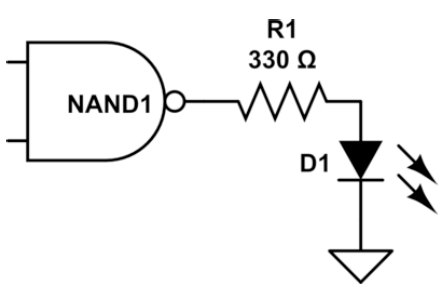
\includegraphics[scale=0.35]{../Figs-Tabs/NEND.png}
	\end{figure}\label{f:NEND}

\begin{table}[htb]
	\centering
	\begin{tabular}{sss}
		\toprule
		\text{ingresso} A & \text{ingresso} B &\text{uscita porta NAND }$\overline{A\cdot B}$	\\
		\midrule
		0  & 0 & 1\\
		0  & 1 & 1\\
		1  & 0 & 1\\
		1  & 1 & 0\\
		\bottomrule
	\end{tabular}
	\caption{Tabella di verità di una porta NEND.}
	\label{t:NEND}
\end{table}

\subsection{osservazione con dip switch}
	Essendo le porte NAND impiegate basate su logica TTL quando esse non risultino collegate a terra si ottiene in uscita un segnale corrispondente allo stato HIGH; cosa che non avviene qualora si abbia un collegamento a terra.
	Si è pertanto procedto a collegare da un lato gli ingressi 1 e 2 del deap switch alla tensione di GROND e da l'altro rispettivamente agli ingressi A e B del NEND.
	
	Il diodo led  essendo acceso qalora l'uscita del NEND sia alta
	e spento qualora  l'uscita sia in stato LOW
	permette la verifica della tabella di verità.
	
	Si è procedto pertanto alla verifica della tabella di verità provando le varie permitazioni degli switch 1 e 2, ottenendo n perfetto accordo con \tablename{ \ref{t:NEND}}.
\subsection{Impiego di Ardino e del oscilloscopio}\label{sez:ard}
	Per effettare una ulteriore verifica di tale tabella di verità 
	si è proceduto a collegare le porte A e B della porta NAND rispettivamente alle 
	uscite Y1 ed Y2 del circuito impulsatore, realizzato con arduino nell'esperienza 10,
	e si  collegata l'uscita della NAND all'oscilloscopio.
	
	Essendo le traccie ottente alle porte Y1 e Y2 dell'impulsatore due onde quadre 
	sfasate relativamente di $\pi/2$ su di un periodo assumono tuttue le permutazioni di due ingressi ad un bit.
	Si riportano le acquisizioni ottente all'oscilloscopio in \figurename{ \ref{f:osci}} .
	\begin{figure}[hb]
		\centering
		\subfloat[acquisizione delle tensioni in ingresso nella porta NEND; A (ch1) ed B (ch2)]{
		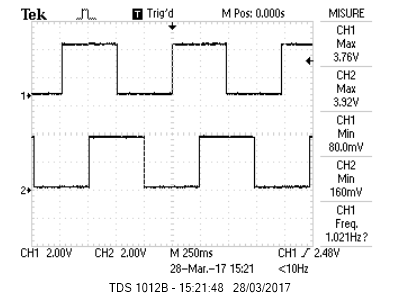
\includegraphics[scale=0.35]{../Figs-Tabs/ingressi.png}
		\label{f:ing}
	}\\
	\subfloat[acquisizione uscita porta NEND (ch2) e della tensione in ingresso A (ch1)]{
		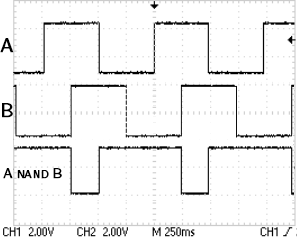
\includegraphics[scale=0.35]{../Figs-Tabs/NAND.png}
		\label{f:sci}
	}\\
	\caption{acquisizioni delle schermate impiegate per la verifica di \tablename{ \ref{t:NEND}}.}
	\label{f:osci}
\end{figure}

	Per rendere significativa l'acquisizione dell'uscita dalla porta NEND ( \figurename{ \ref{f:sci}} ) si è acquisito contemporaneamente uno dei de ingressi, nella fattispecie A; dopodiché si sono acquisiti entrambi i segnali  in ingresso (\figurename{ \ref{f:ing}} ) quale indicazione dello stato di ingresso.
	
	Dall'osservazione della \figurename{ \ref{f:osci}} si ottiene un ulteriore verifica della \tablename{ \ref{t:NEND}}.
\section{Progettazione e verifica semplici circiti logici}
	Per verificare le tabelle di verità dei seguenti circuiti si è impiegato il circuito impulsatore; ed in particolare la tecnica descritta in\textbf{ sezione \ref{sez:ard} }.
	Si segnala che per tutta la sezione verrà impiegata la \figurename{ \ref{f:ing}} quale riferimento per i segnali in ingresso.
	\subsection{AND}
	Per verificare l'andamento di un circuito AND, essendo
	$$AND(A,B) = A \cdot B = \overline{(\overline{A \cdot B})}$$
	si è montato il circuito in \figurename{ \ref{f:AND}} 
	\begin{figure}[htb]
		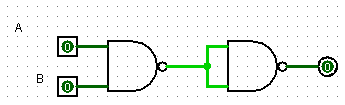
\includegraphics[scale=1.0]{../Figs-Tabs/ENd.png}
		\caption{rappresentazione di un circito AND realizzato con porte NAND. A e B rappresentano gli ingressi mentre si campiona in scita sl terzo terminale.}
	\end{figure}\label{f:AND}
.
	Tale circito presenta la tabella di verità riportata in \tablename{ \ref{t:AND}} 
	\begin{table}[htb]
		\centering
		\begin{tabular}{sss}
			\toprule
			\text{ingresso} A & \text{ingresso} B &\text{uscita porta AND }$A\cdot B$	\\
			\midrule
			0  & 0 & 0\\
			0  & 1 & 0\\
			1  & 0 & 0\\
			1  & 1 & 1\\
			\bottomrule
		\end{tabular}
		\caption{Tabella di verità di una porta AND.}
		\label{t:AND}
	\end{table}.
	la quale risulta a sua volta verificata dall'andamento osservato
	e riportato in \figurename{ \ref{f:osci-and}}
	
	\begin{figure}[hb]
		\centering
		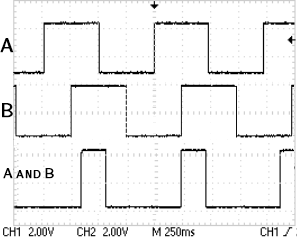
\includegraphics[scale=0.35]{../Figs-Tabs/and.png}
		\caption{acqusizione della schermata impiegata per la verifica di \tablename{ \ref{t:AND}}.
		Uscita funzione AND (ch2) e tensione in ingresso in A (ch1).
		}
		\label{f:osci-and}
	\end{figure}.
	\subsection{OR}
			Per la funzione OR essendo $$ OR(A,B) = A + B = \overline{\overline{(A +B)}}= \overline{(\overline{A} \cdot \overline{B})}$$
			è stato montato il circuito in \figurename{ \ref{f:OR}} 
		\begin{figure}[htb]
			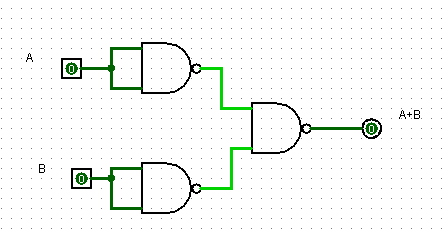
\includegraphics[scale=1.0]{../Figs-Tabs/OR2.png}
			\caption{rappresentazione di un circito OR realizzato con porte NAND. A e B rappresentano gli ingressi mentre si campiona in uscita sul terzo terminale.}
		\end{figure}\label{f:OR}.
		Tale circito presenta la tabella di verità riportata in \tablename{ \ref{t:OR}} 
		\begin{table}[htb]
			\centering
			\begin{tabular}{sss}
				\toprule
				\text{ingresso} A & \text{ingresso} B &\text{uscita porta AND }$A\cdot B$	\\
				\midrule
				0  & 0 & 0\\
				0  & 1 & 1\\
				1  & 0 & 1\\
				1  & 1 & 1\\
				\bottomrule
			\end{tabular}
			\caption{Tabella di verità di un circito OR.}
			\label{t:OR}
		\end{table}.
		la quale risulta a sua volta verificata dall'andamento osservato
		e riportato in \figurename{ \ref{f:osci-or}}
		
		\begin{figure}[hb]
			\centering
			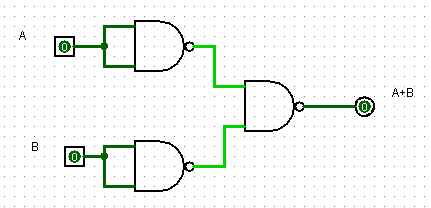
\includegraphics[scale=0.35]{../Figs-Tabs/or.png}
			\caption{acquisizione della schermata impiegata per la verifica di \tablename{ \ref{t:OR}}.
				Uscita circito OR (ch2) e tensione in ingresso in A (ch1).
			}
			\label{f:osci-or}
		\end{figure}.
	\subsection{XOR}
	Per la funzione XOR essendo $$ XOR(A,B) = A \oplus B = (A \cdot \overline{B}) + (\overline{A} \cdot B) =
	 \overline{
	 	\overline{
	 		( A \cdot \overline{
	 			(A \cdot B) )
 			}	\cdot 
 		\overline{
 			(B \cdot \overline{
 				(A \cdot B)
 			} )
 		}
 	}
	}$$
	è stato montato il circuito in \figurename{ \ref{f:XOR}} 
	\begin{figure}[htb]
		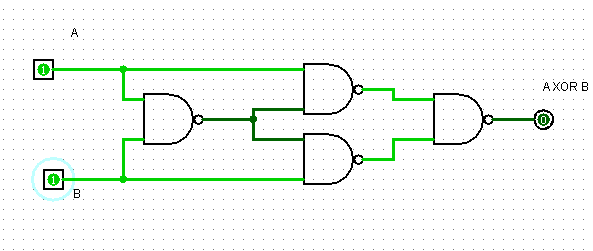
\includegraphics[scale=1.0]{../Figs-Tabs/XOR2.png}
		\caption{rappresentazione di un circuito XOR realizzato con porte NAND. A e B rappresentano gli ingressi mentre si campiona in uscita sul terzo terminale.}
	\end{figure}\label{f:XOR}.
	Tale circuito presenta la tabella di verità riportata in \tablename{ \ref{t:XOR}} 
	\begin{table}[htb]
		\centering
		\begin{tabular}{sss}
			\toprule
			\text{ingresso} A & \text{ingresso} B &\text{uscita porta XOR }$A \oplus B$	\\
			\midrule
			0  & 0 & 0\\
			0  & 1 & 1\\
			1  & 0 & 1\\
			1  & 1 & 0\\
			\bottomrule
		\end{tabular}
		\caption{Tabella di verità di un circito XOR.}
		\label{t:XOR}
	\end{table}.
	la quale risulta a sua volta verificata dall'andamento osservato
	e riportato in \figurename{ \ref{f:osci-xor}}
	
	\begin{figure}[hb]
		\centering
		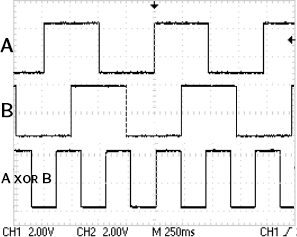
\includegraphics[scale=0.35]{../Figs-Tabs/xor.png}
		\caption{acqusizione della schermata impiegata per la verifica di \tablename{ \ref{t:XOR}}.
			Uscita circito XOR (ch2); tensione in ingresso in A (ch1).
		}
		\label{f:osci-xor}
	\end{figure}.
\subsection{Circito sommatore ad un bit}	
	Per realizzare il circuito sommatore richiesto si è assunto
	che esso potesse costituirsi su un uscita [uscita 1] di una funzione XOR, per esprimere il bit più significativo;
	ed da una funzione AND sull uscita rimanente [uscita 2] per esprimere il meno significativo.
	Si è montato pertantonto il circito in \figurename{ \ref{f:somma}}.
		\begin{figure}[htb]
		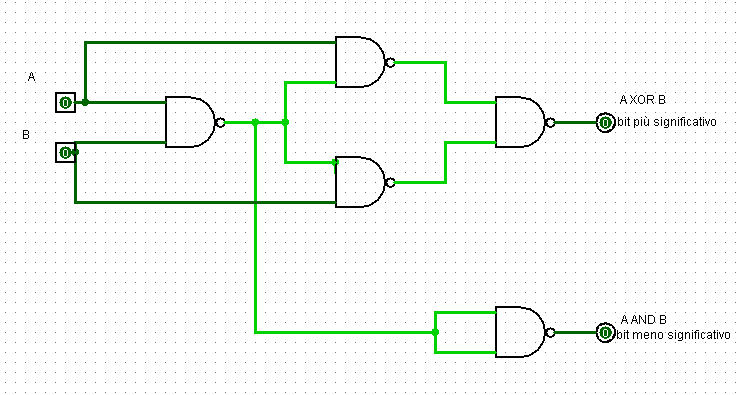
\includegraphics[scale=1.0]{../Figs-Tabs/somma.png}
		\caption{rappresentazione di un circito sommatore a 2 ingressi e 2 uscite.}
	\end{figure}\label{f:somma}
	
	L'andamento del circito risulta verificato dalla 	\figurename{ \ref{f:osci-somma}}.
	
	\begin{figure}[hb]
	\centering
	\subfloat[acqsizione della tensione in uscita dal circito XOR (ch2) ed in ingresso A (ch1);
	tale figura costituisce insieme alla \figurename{ \ref{f:ing}} un riferimento]{
		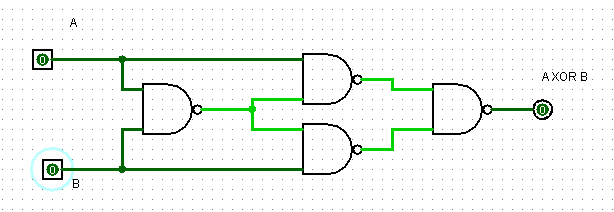
\includegraphics[scale=0.35]{../Figs-Tabs/XOR.png}
		\label{f:ing-somma}
	}\\
	\subfloat[acquisizione delle tensioni in uscita dal circito XOR (ch2) ed in uscita dal circito AND (ch1)]{
		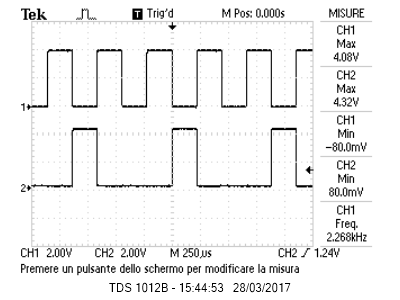
\includegraphics[scale=0.35]{../Figs-Tabs/sommatore_out.png}
		\label{f:sci-somma}
	}\\
	\caption{acqusizioni delle schermate impiegate per la verifica del funzionamento del circuito sommatore.}
	\label{f:osci-somma}
\end{figure}
Si può infatti osservare che l'uscita assuma alternativamente i valori $00-01-10-11$.


\section{Generatore di onda quadra}
	Per la realizzazione di un generatore di onda quadra
	si sono impiegati i circuiti impiegati per il multivibratore monostabile e
	per il multivibratore astabile 
	accoppiandoli in maniera da ottenere il da ottenere il circuito in \figurename{ \ref{f:qadra}}.
	\begin{figure}[htb]
		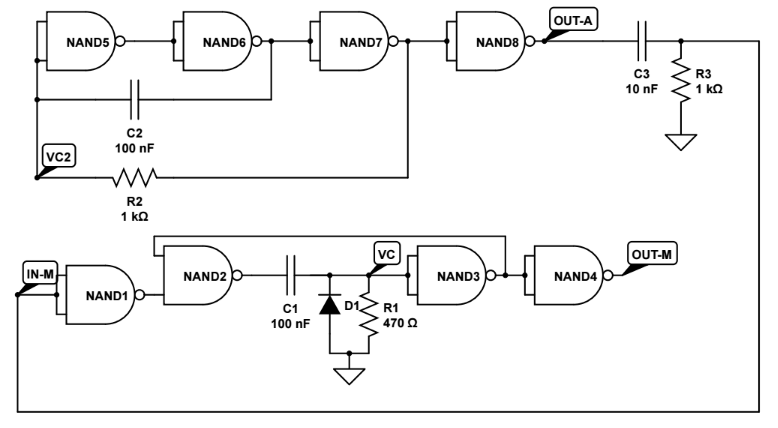
\includegraphics[scale=1.0]{../Figs-Tabs/qadra.png}
		\caption{rappresentazione del circuito realizzato per generare un onda quadra.}
	\end{figure}\label{f:qadra}

	Per il montaggio circuitale sono state impiegate le seguenti componenti\footnote{Tali valori sono stati ottenuti attraverso il multimetro digitale in dotazione. A tali misure sono state associate le incertezze calcolate sommando in quadratura l'errore di lettura con l'errore di calibrazione dello strumento.} :\\
	\begin{center}
		$R_{3}=$\SI{988 \pm 8}{\ohm}\\
		$C_{3}=$\SI{10.8 \pm 0.4 }{\nano \farad}\\
	\end{center}
	
	Si riportano in \figurename{ \ref{f:osci-qad}} l'acquisizione del segnale in 
	ingresso nel multivibratore monostabile; ovvero il segnale in uscita dal derivatore (ch2) ed il segnale in ingresso (ch1).
	\begin{figure}[htb]
		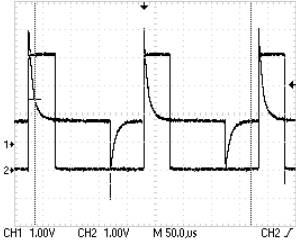
\includegraphics[scale=1.0]{../Figs-Tabs/deth_generator.png}
		\caption{Acquisizione dei segnali in ingresso [ch1] ed in uscita [ch2] dal circuito monostabile.}
	\end{figure}\label{f:osci-qad}
	Il circuito monostabile, come riscontrabile in \figurename{ \ref{f:osci-qad}},
	trasforma l'onda quadra generata dall'astabile in un impulso di breve durata temporale; sempre dalla figura in esame può essere osservato che il monostabile risulti sensibile al fronte di salita del segnale in ingresso.
	
	Come atteso, dall'andamento osservato in sezione 2, in uscita al circuito monostabile si ottiene un onda quadra [ch2 di \figurename{ \ref{f:osci-qad}}].
	Tale onda presenta un periodo 
	$T=$\SI{205 \pm 1 }{\mu \sec}
	\footnote{valori misurati con i cursori dell'oscilloscopio. Si è associata l'incertezza dovuta all'errore di posizionamento dei cursori; a cui si aggiunge a parte l'errore di calibrazione dello strumento.}
	a fronte di un impulso di $\Delta T_{up} =$\SI{47.0 \pm 0.2 }{\mu \sec}
	\footnote[1]{}
	Si ottiene pertanto un duty-cycle $\frac{\Delta T_{up}}{T}= 22.9 \pm 0.2$\textdiscount.
	
	Nella sezione 2 è stato osservato che l'impulso ,$\Delta T_{up}$, 
	abbia una dipendenza lineare dal valore della resistenza $R_{2}$;
	la durata del periodo ne risulti indipendente; poiché non varia apprezzabilmente al variare di $R_{2}$.
	
	Mentre nella sezione  è stata osservata la dipendenza lineare 
	del periodo $T$ dal valore della resistenza $R_{1}$;
	mentre la durata del impulso non vari significativamente.
	
	Si assume pertanto che $$ \Delta T_{up} \propto R_{2}$$
		$$T \propto R_{1} $$
	e non il viceversa.
	Per la verifica di tale assunzione si è proceduto a variare separatamente i valori di $R_{1}$ e $R_{2}$; si ottengono i dati in \tablename{ \ref{t:4}}.
		
	\begin{table}[htb]
		\centering
		\begin{tabular}{*{5}{S}}
			\toprule
			$R_{1}$ [\si{\ohm}] & $R_{2}$ [\si{\kilo \ohm}] & $T$ [\si{\mu \sec}] & $\Delta T_{up}$  [\si{\mu \sec}] & $\frac{\Delta T_{up}}{T}$ \\
			\midrule
			470\pm 5	&	1.12 \pm 0.01	&	234 \pm 1	&	47.6\pm2	&	4.92 \pm3	\\ 
			567 \pm6	&	1.12 \pm 0.01	&	234\pm1	&	59.2 \pm4	&	3.95\pm 0.03	\\ 
			567 \pm6	&	0.988 \pm 0.009	&	205\pm1	&	59.2 \pm0.4	&	3.46\pm0.03	\\ 
			\bottomrule
		\end{tabular}
		\caption{
			Tabella dei valori campionati per la verifica delle dipendenze di $\Delta T_{up}$ e $T$ dai valori di $R_{1}$ e  $R_{2}$.
		}
		\label{t:4}
	\end{table}
	Come possiamo osservare dai valori tabulati si ottiene un sostanziale accordo con la proporzionalità attesa.
	
	Si è adesso proceduto a realizzare un generatore di onde quadre di $T_{att}\sim 100$\si{\mu \sec} e $ \Delta {T_{up}}_{att}\sim 30$\si{\mu \sec}.
	
	Dai valori ottenuti nelle sezioni 2 e 3 e  dai rispettivi coefficienti stimati $a=$ e $b=$
		abbiamo stimato per i valori richiesti delle resistenze attese 
	${R_{2}}_{att}=$\SI{470 \pm 30}{\ohm}%valore placeholder
	${R_{1}}_{att}=$\SI{260 \pm 40}{\ohm}%valore placeholder.
	Si è osservato tuttavia che impiegando tali resistori si ottiene un impulso sensibilmente diverso da quello atteso.
	Si è pertanto proceduto a variare i valori delle resistenze sino ad ottenere un accordo tra i valori misurati e quanto richiesto.
	Al termine di tale processo sono state impiegate delle resistenze 
	$R_{1}=$\SI{331 \pm 3}{\ohm}
	$R_{2}=$\SI{464 \pm 4}{\ohm}
	ottenendo 
	$T=$\SI{101 \pm 1}{\mu \sec} e $ \Delta {T_{up}}=$\SI{30.2 \pm 0.2}{\mu \sec}.
	
	Una posssibile causa della discrepanza tra i valori dei resistori, per cui si verifichi l'accordo con le richieste, ed  i valori di ${R_{2}}_{att}$ e 	${R_{1}}_{att}$ potrebbe essere imputabile ad un andamento non esattamente lineare nelle dipendenze di $ \Delta T_{up}$ da $ R_{2}$ e di
	$T $ da $ R_{1} $
	
	
	
	
	
	
	
	
	
	
\section{Misura di \textbf{r}}

Dopo aver misurato $B$ si inserisce il bulbo nell'alloggiamento posto tra le bobine.
Si alimenta il filamento interno con una tensione sufficiente alla produzione di elettroni per effetto termoionico, si procede quindi all'alimentazione delle bobine di Helmholtz (tra \SI{6}{\volt} e \SI{9}{\volt}) e del cannone elettronico (tra \SI{200}{\volt} e \SI{300}{\volt}).
	
%Per i valori di $V_{coil}$ e $V_{acc}$ appena fissati si è  osservata la variazione del pennellino elettronico al variare di 	$V_{heat}$.
%Per valori di $V_{heat}<$\SI{3}{\volt}
%non si osserva emissione di \e; ciò suggerisce la presenza di un valore di soglia
%$\sim 3 V$. Per valori $V_{heat}>$\SI{3}{\volt} ma ad esso prossimo
%si osserva che il fascio sia meno definito rispetto alle tensioni superiori;
%qesto effetto rislta compatibile col fatto che il filamento si trovi ,o termalizzi, a temperatre più basse qindi emetta %meno \e;

Si posiziona la reflex con l'asse dell'obiettivo perpendicolare al piano in cui si muovono gli elettroni, centrato rispetto al centro del bulbo.
Si procede quindi ad acquisire foto dell'apparato al variare di $B$ (controllato variando la tensione di alimentazione delle bobine e misurando $I$) e $V$ nei range sopra descritti.

In \figurename{ \ref{f:acquisizione}} si riportano alcune delle foto acquisite a titolo di esempio.
		
		\begin{figure}[H]
		\centering
		\subfloat{
			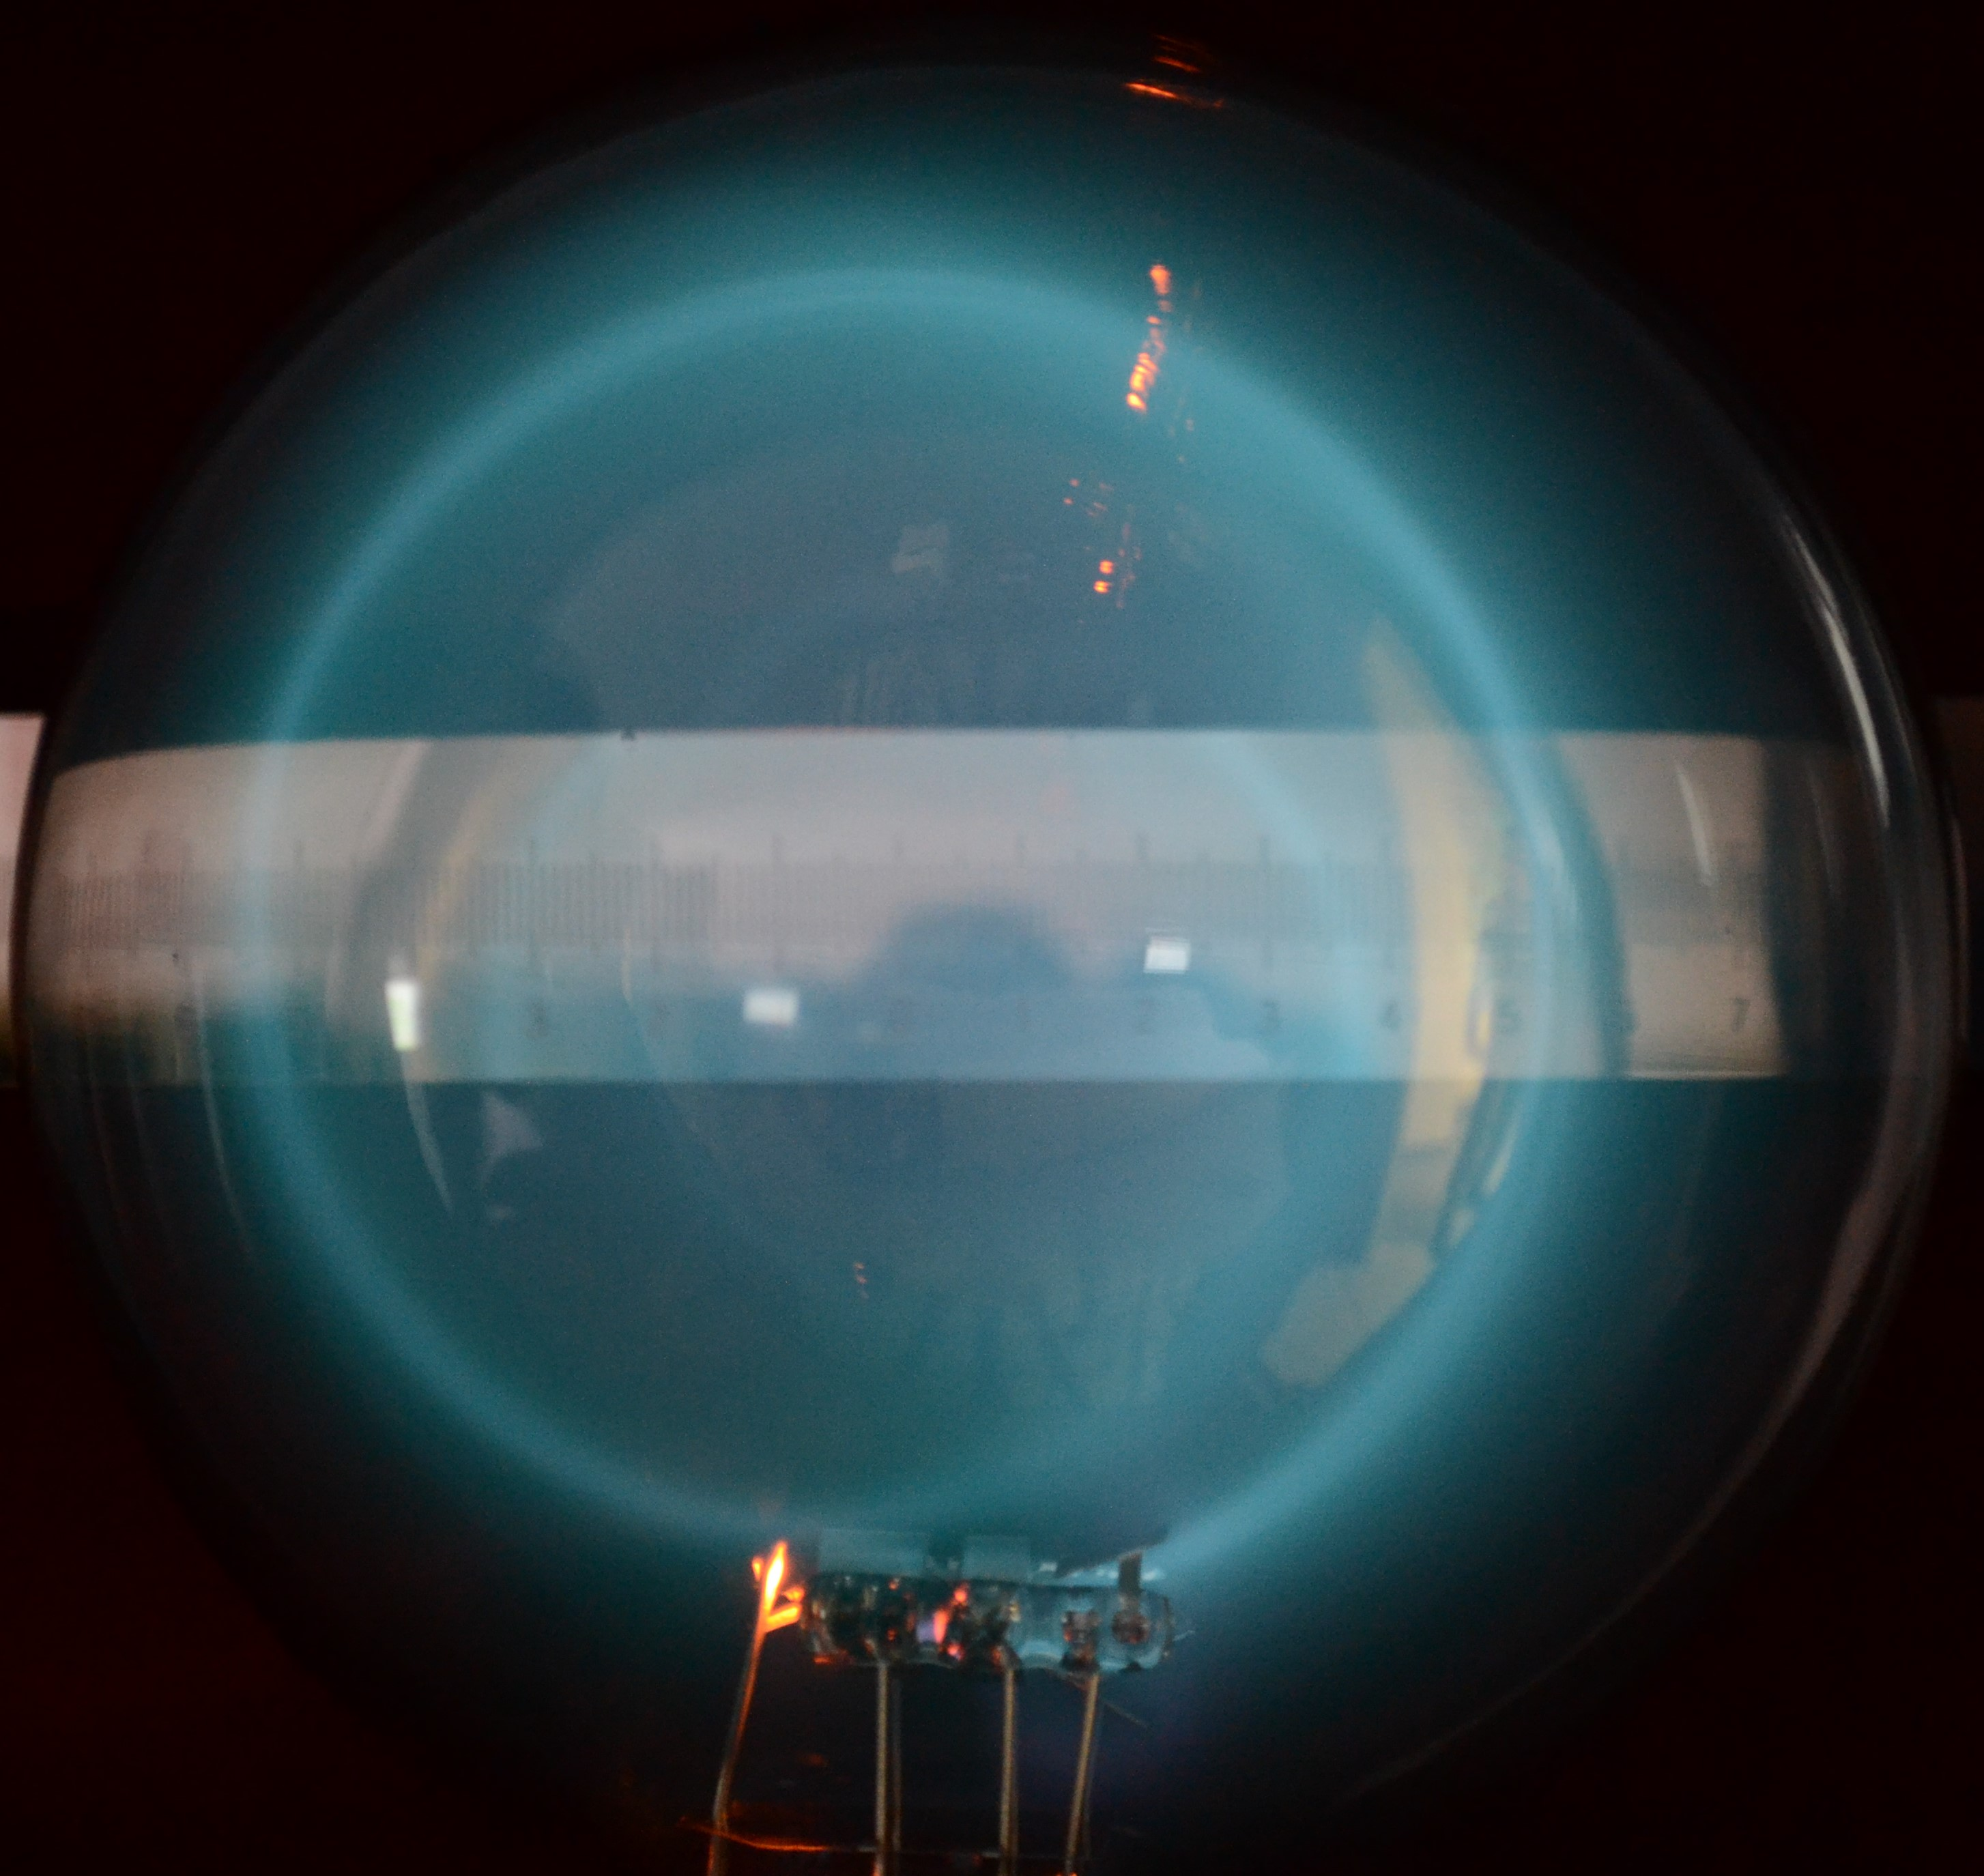
\includegraphics[scale=0.30]{(11).JPG}
			\label{stocazzo}}
		\subfloat{
			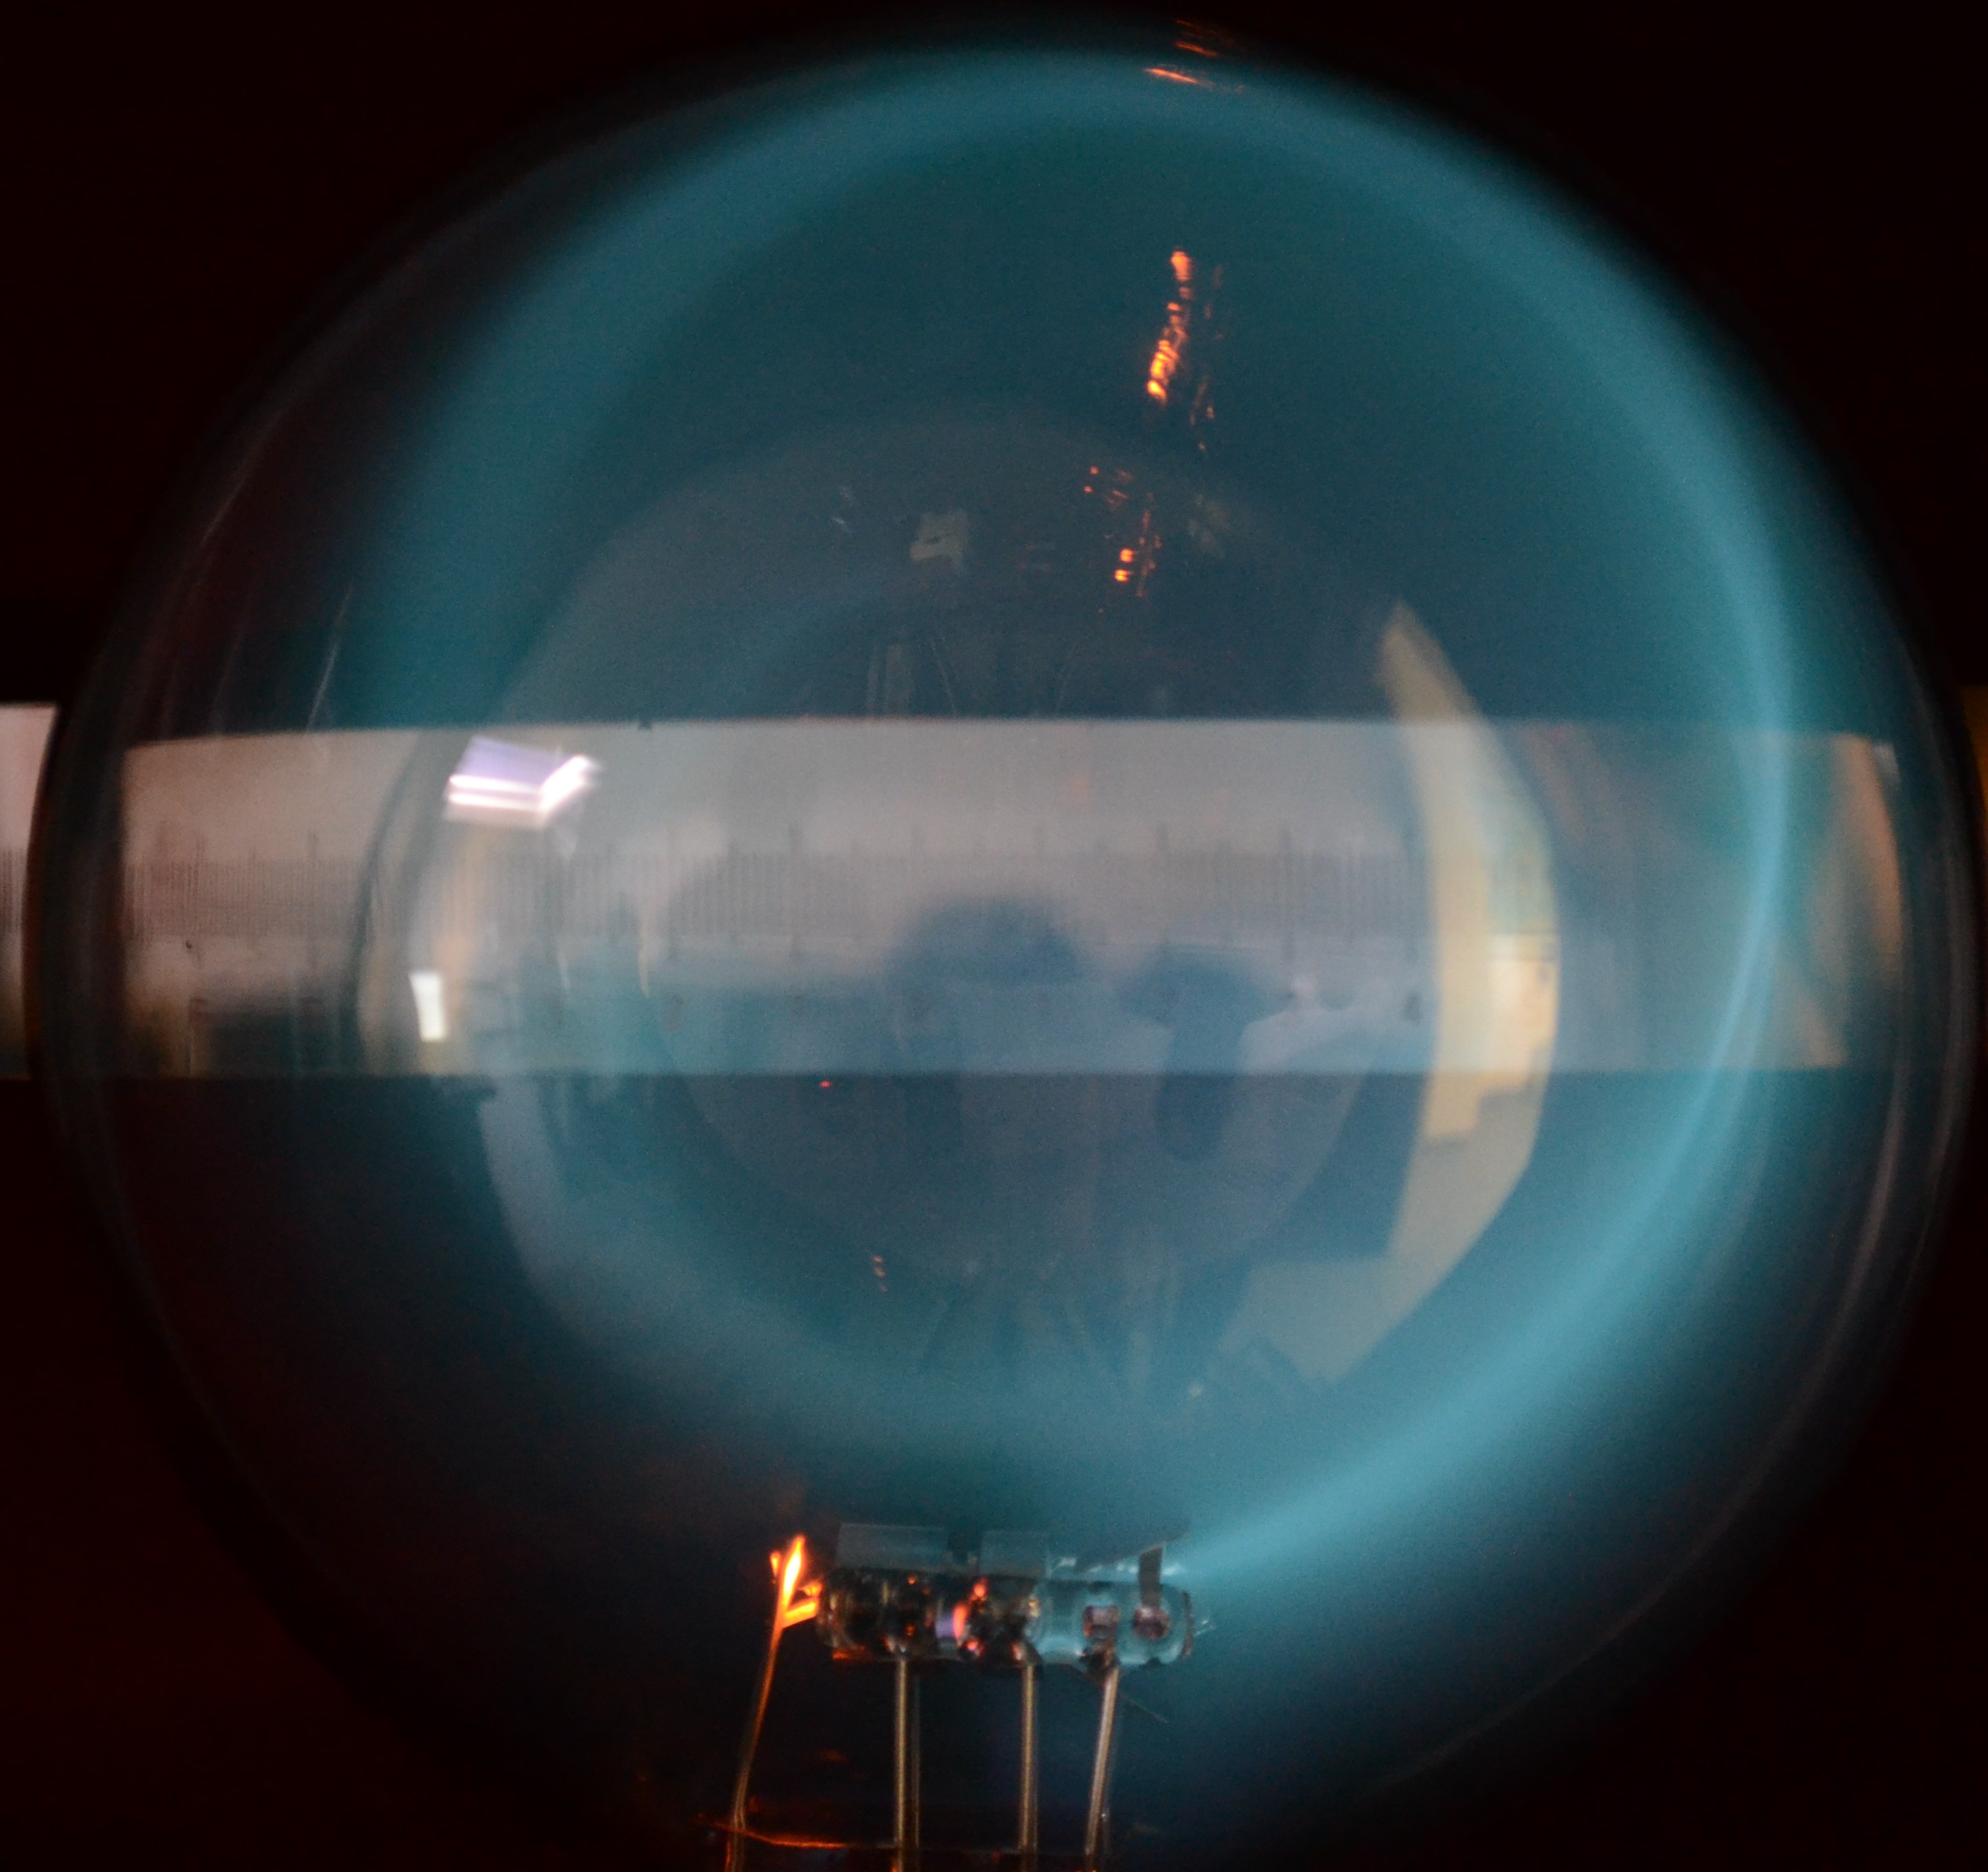
\includegraphics[scale=0.303]{(1).JPG}
			\label{coda}}\\
		\subfloat{
			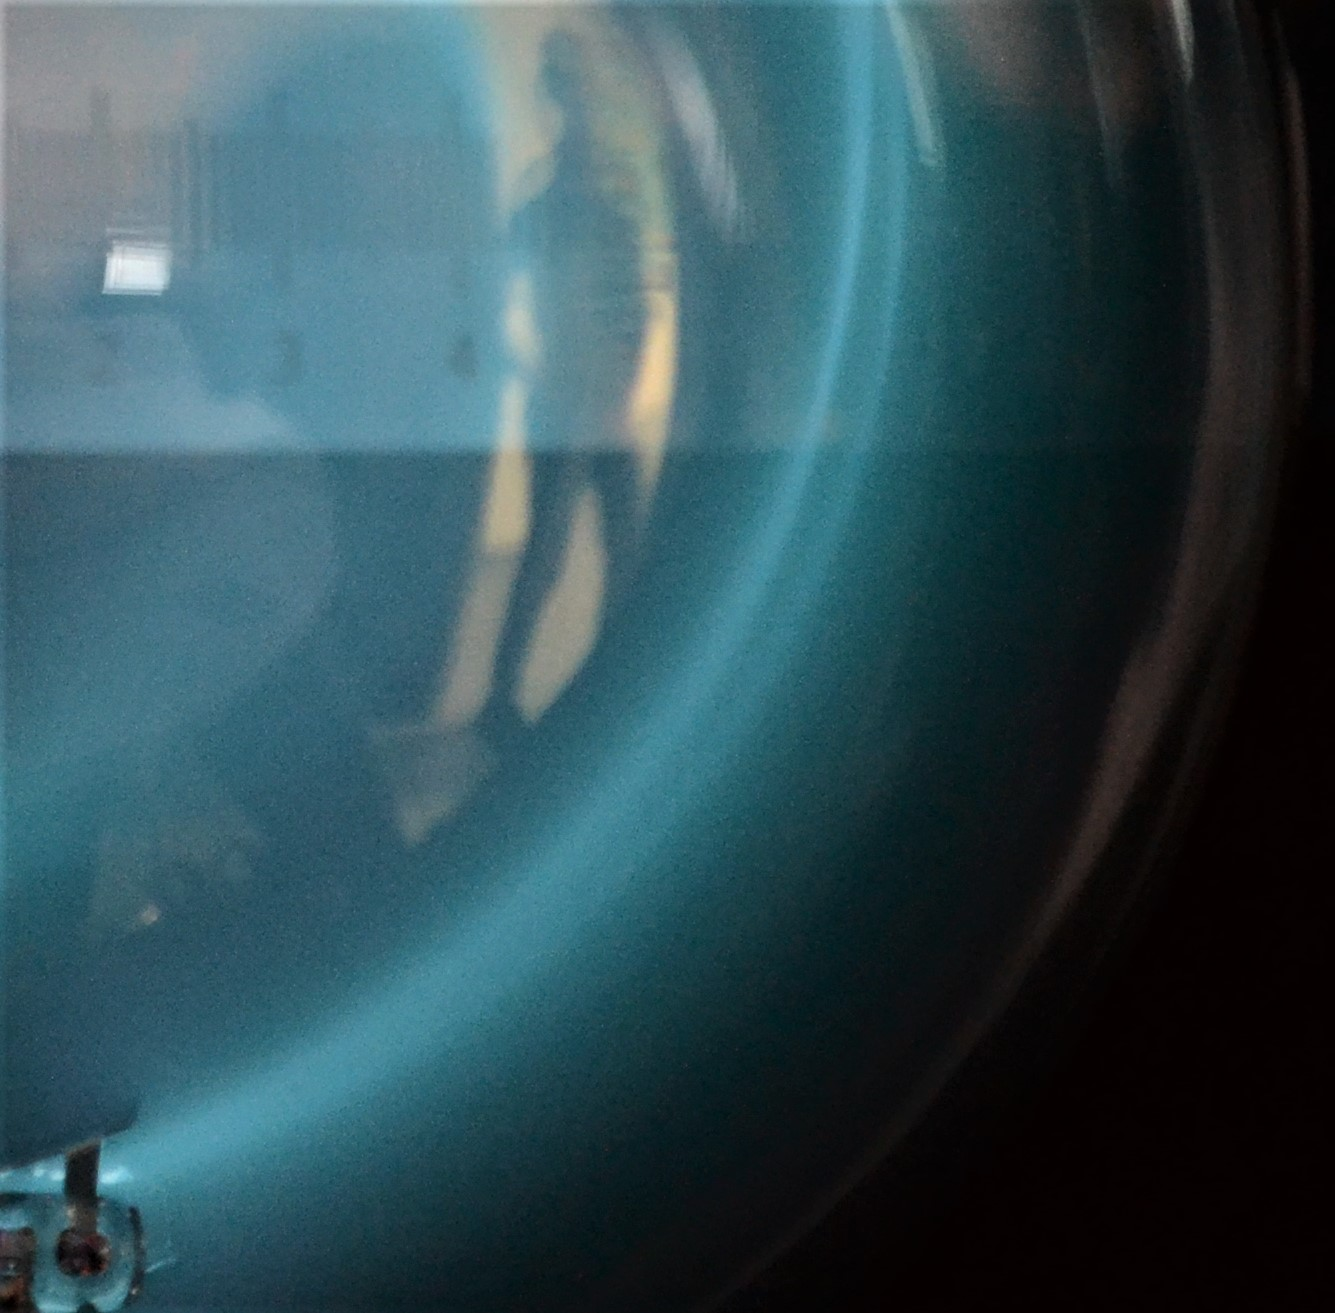
\includegraphics[scale=0.639]{(18).JPG}
			\label{doppio}}
		\subfloat{
			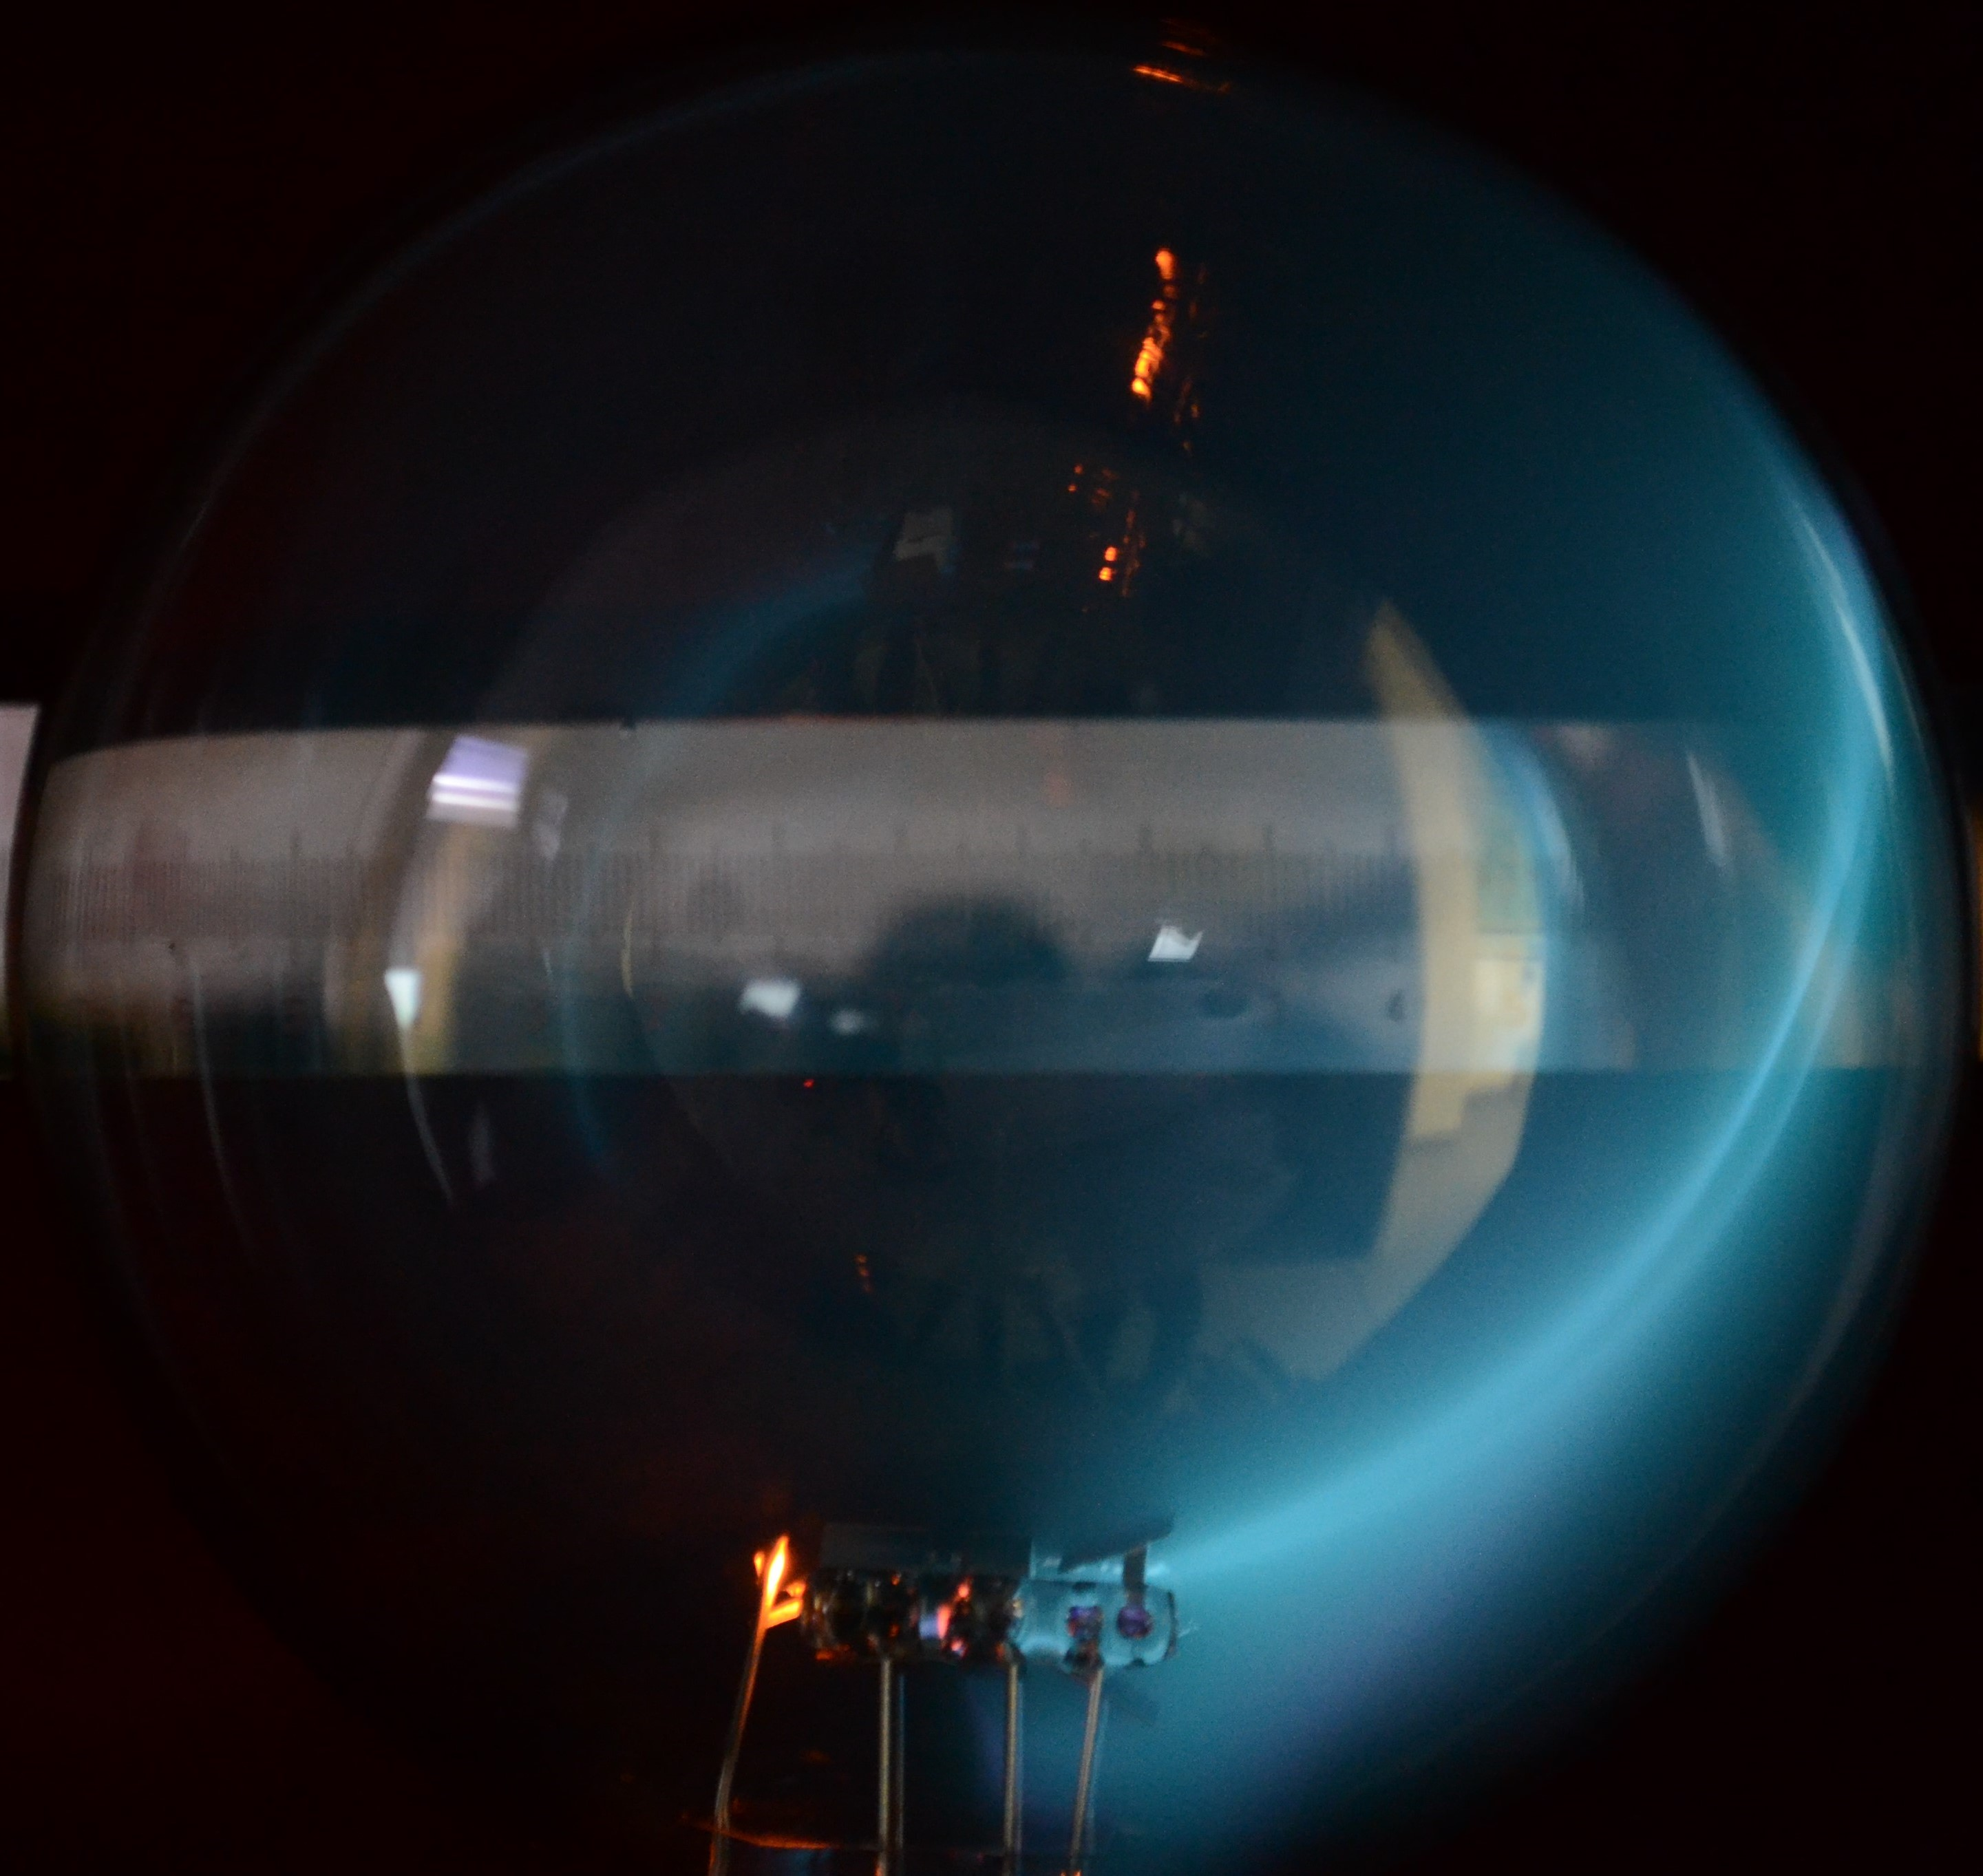
\includegraphics[scale=0.308]{(60).JPG}
			\label{esce}}
		\caption{Esempi di acquisizioni e anomalie}
		\label{f:acquisizione}
	\end{figure}

Dalle foto si possono notare alcuni elementi di cui bisognerà tener conto durante l'analisi:
\begin{itemize}
	\item il fascio, sopratutto per basse tensioni $V$ del cannone elettronico (e conseguentemente basse energie degli elettroni) si affievolisce velocemente per colpa degli urti tra elettroni e atomi di He nel bulbo, questo rende il fascio dai contorni meno netti e aumenta l'incertezza sulla determinazione del raggio;
	\item nelle stesse condizioni del punto precedente il fascio diminuisce evidentemente il raggio di curvatura poiché gli elettroni perdendo energia curvano di più;
	\item il fascio non è ben collimato, in certi punti è visibile come si divida in due parti, aumentando l'incertezza sulla determinazione del raggio;
	\item per alte tensioni $V$ del cannone elettronico ma basse correnti $I$ passanti per le bobine il fascio esce subito dal bulbo, in queste condizioni la porzione di circonferenza visibile è ridotta e si trova tutta sul bordo del bulbo: la parte più soggetta alle distorsioni ottiche dovute allo stesso.
\end{itemize}

Nel seguito si è tenuto conto di questi effetti, ad esempio ignorando la parte finale della traiettoria o scartando le acquisizioni dove è visibile una parte troppo piccola di circonferenza.

In prima battuta fitteremo le circonferenze misurandone il raggio in pixel, quindi valuteremo il fattore di conversione pixel/metri.

\subsection{Fit delle circonferenze} 
Dato l'elevato numero di foto acquisite si è deciso di procedere ad un fit automatico delle circonferenze. Il procedimento seguito consta di due fasi:
\begin{itemize}
	\item eliminare dalla foto tutti gli elementi estranei alla circonferenza da fittare;
	\item eseguire il fit vero e proprio e valutare l'errore sul raggio.
\end{itemize}

\paragraph{Isolamento delle circonferenze} Si è sfruttato l'alto contrasto delle circonferenze e il loro colore (gli atomi di Elio eccitati emettono per lo più nel blu) per isolarle rispetto agli altri elementi. Utilizzando un software di photo-editing si sono eliminati i canali rosso e verde e tutti i pixel che non avessero luminosità in un certo range (scelto in modo da isolare le sole circonferenze). 

Alla fine di questo procedimento in certe foto è rimasto del segnale riflesso dal righello specchiato che è stato rimosso manualmente.

Un esempio del risultato finale è visibile in \figurename{ \ref{circ}}.

\begin{figure}[H]
	\centering
		\subfloat{
			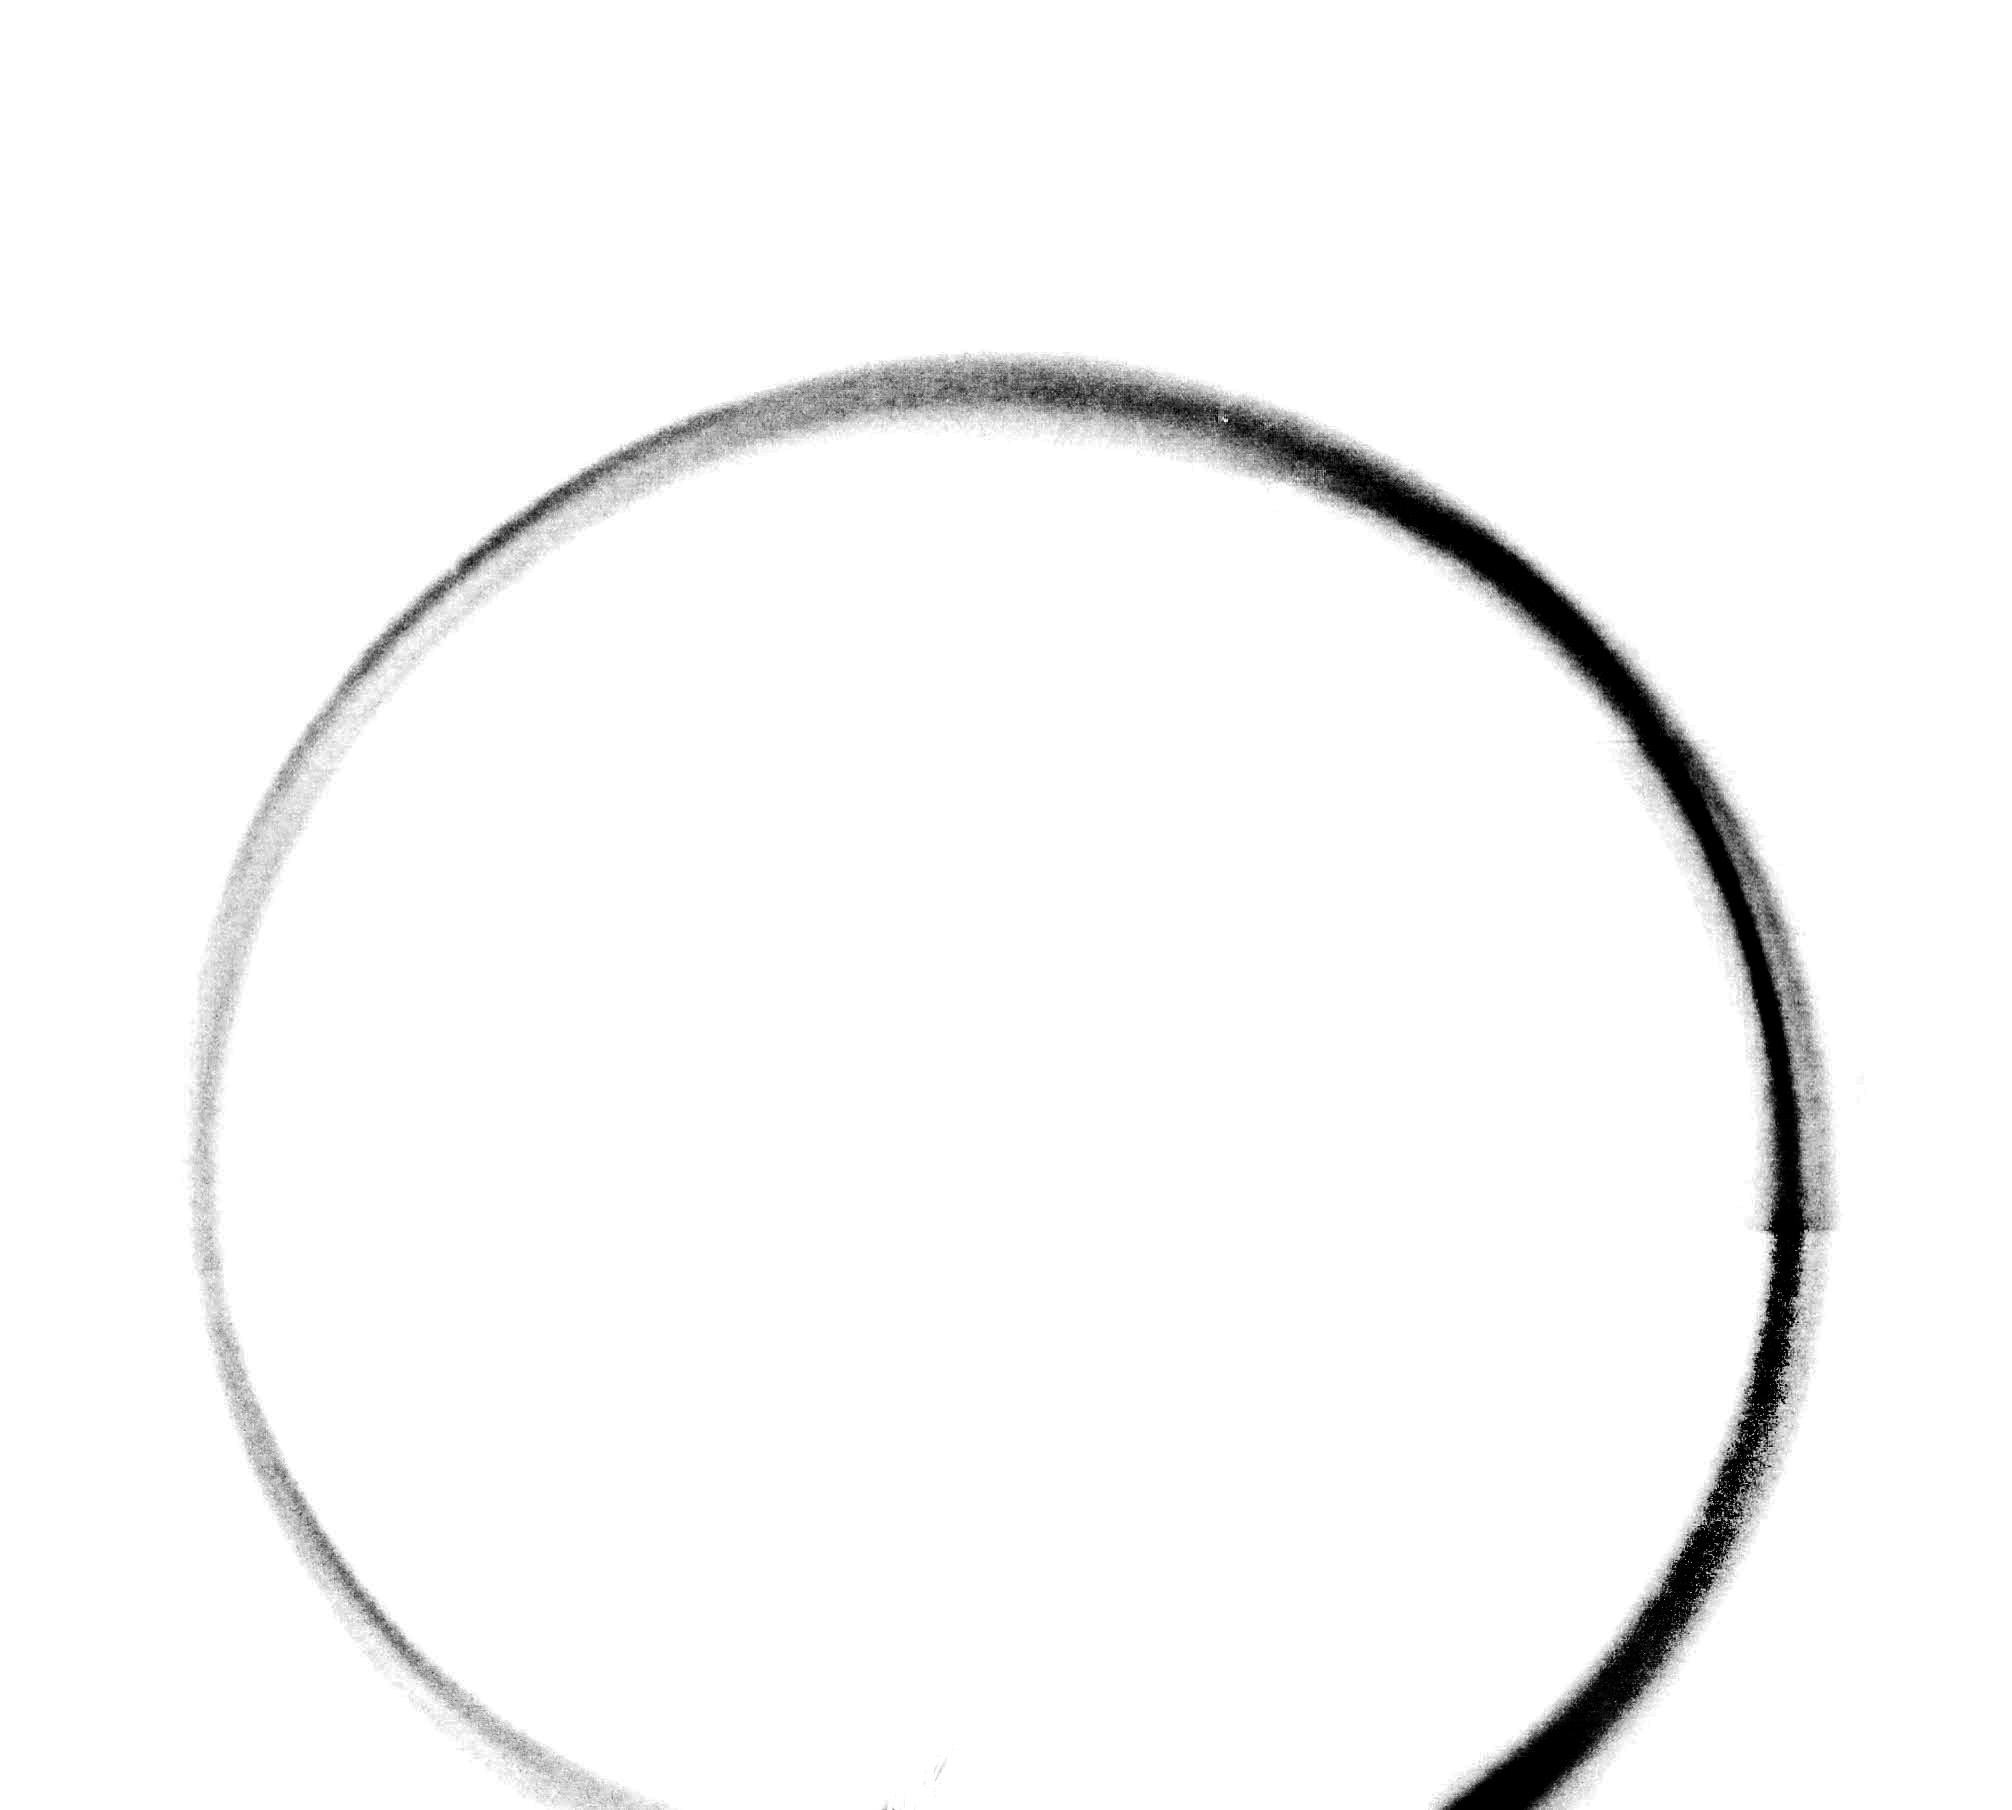
\includegraphics[scale=0.45]{1.JPG}}
		\subfloat{
			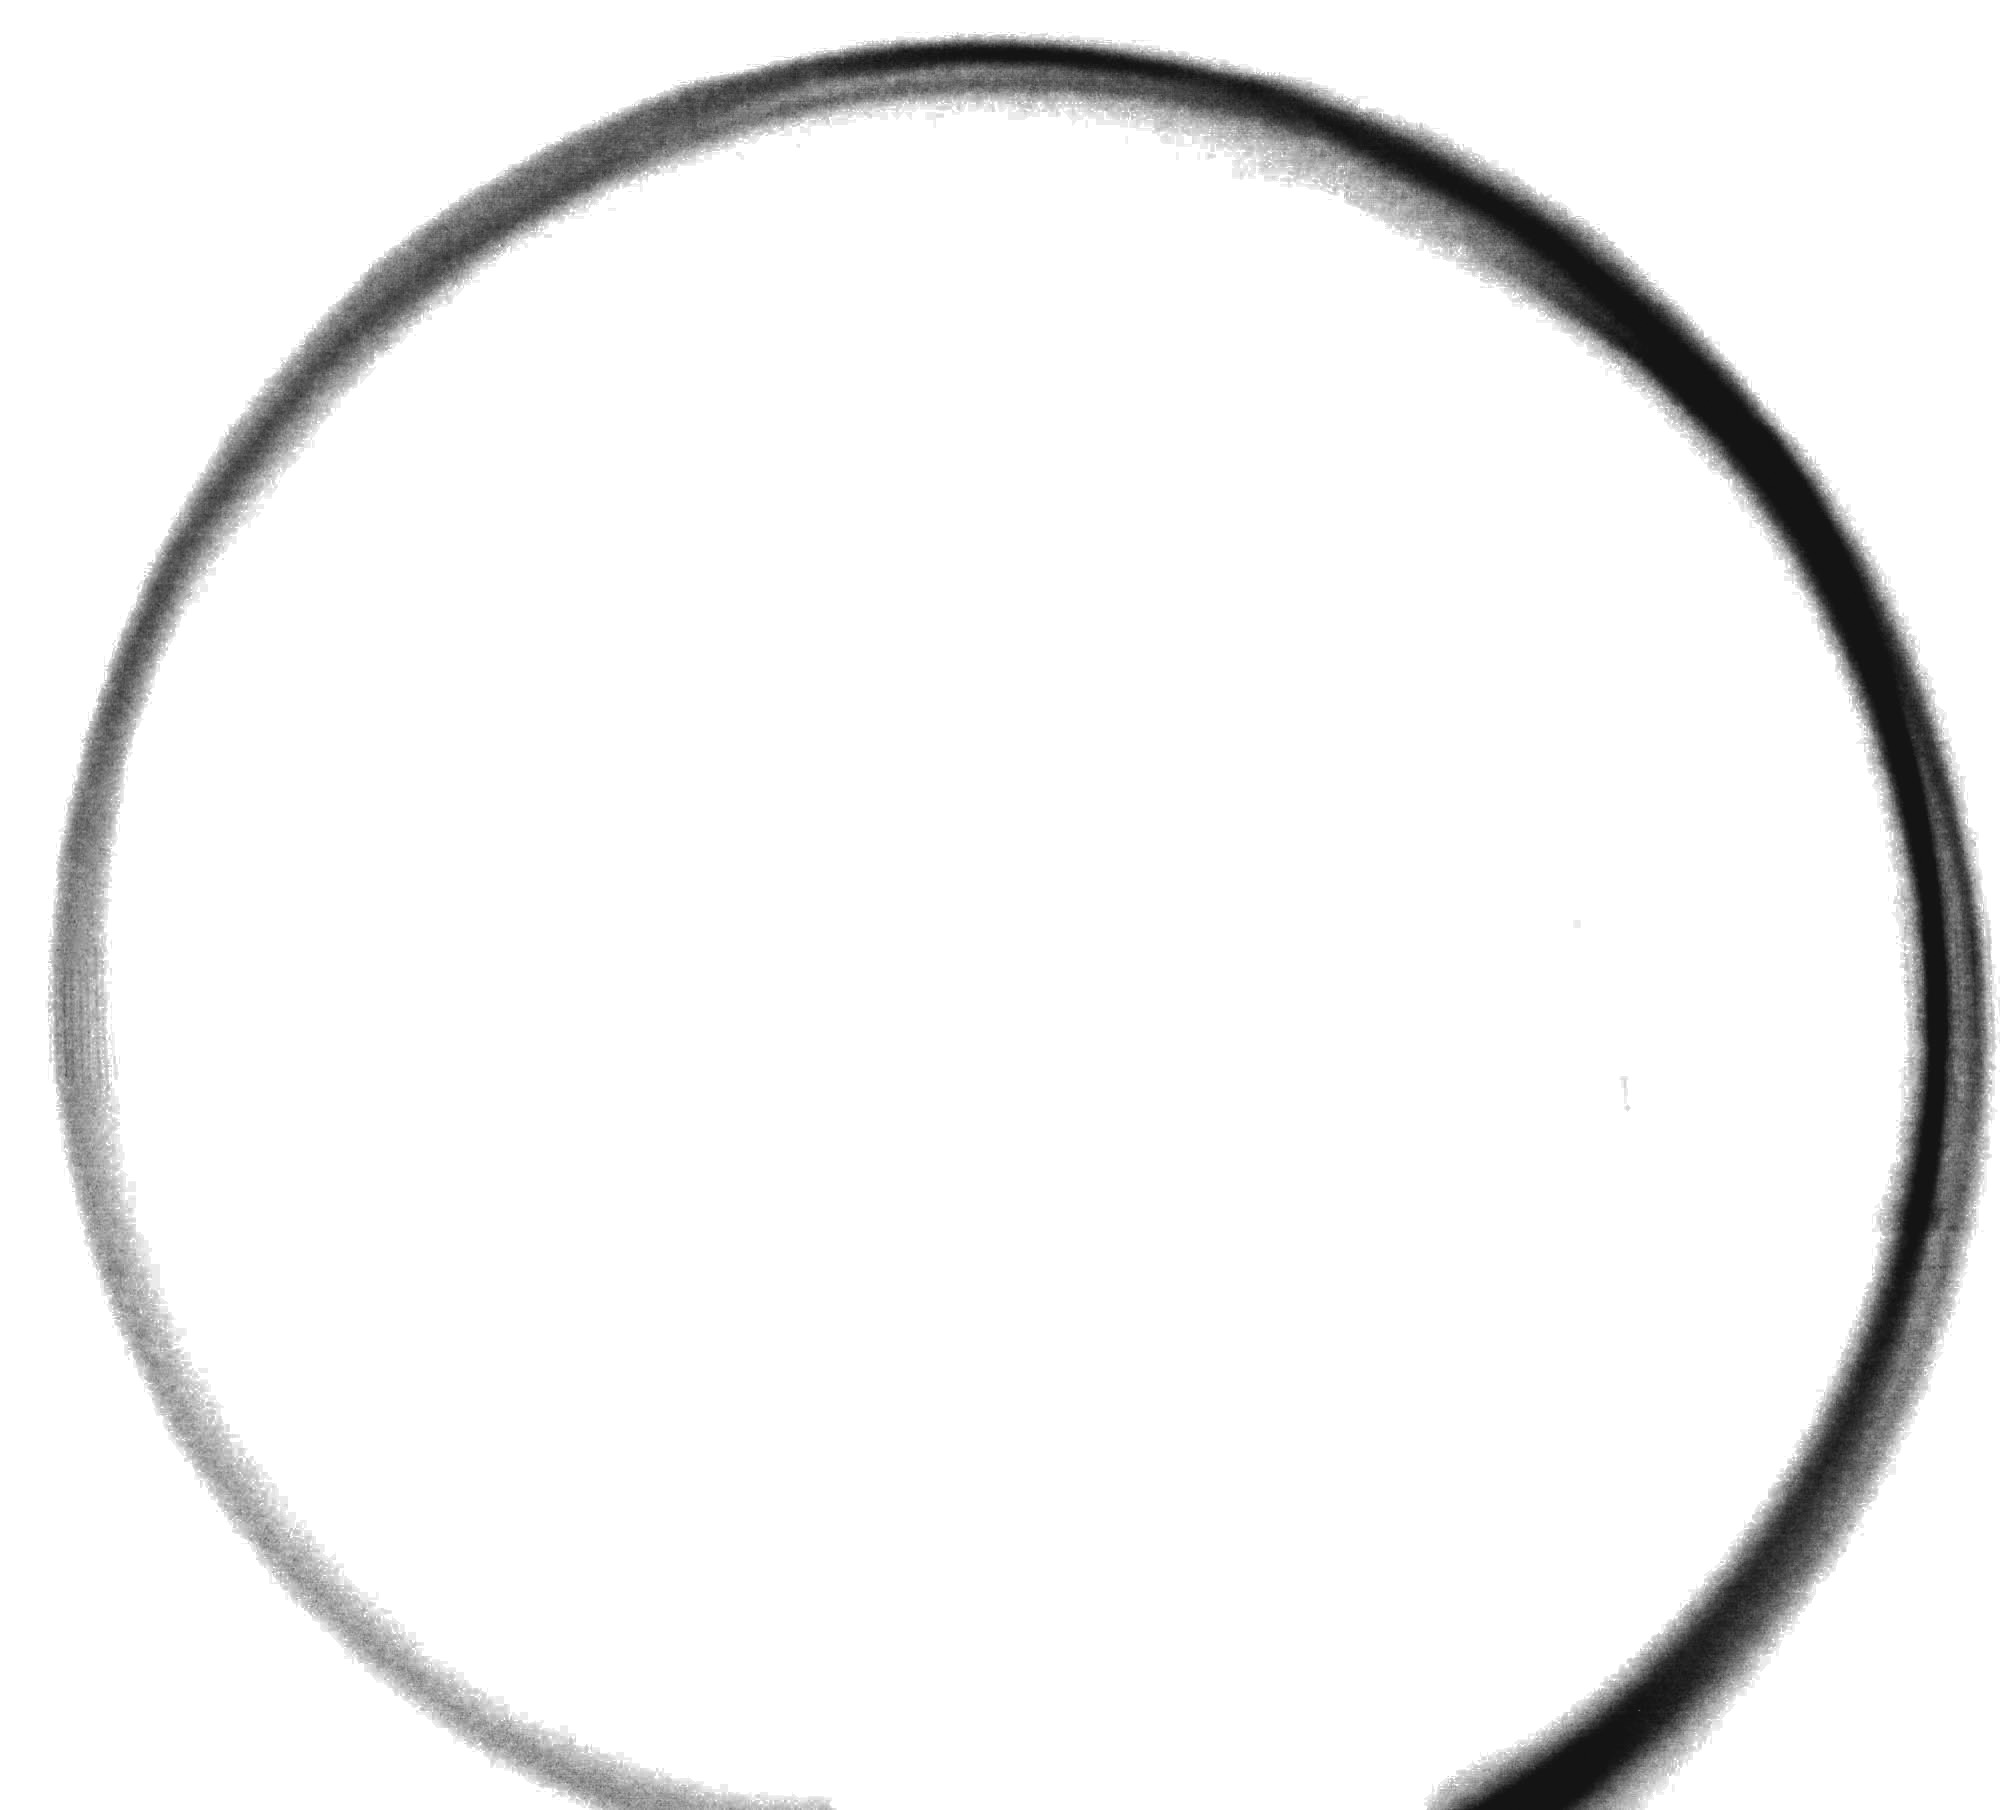
\includegraphics[scale=0.45]{2.JPG}}
	\caption{circonferenze isolate dal background}
	\label{circ}
\end{figure}
%le foto che ho messo non sono nostre, ma di un altro gruppo, ma erano più belline delle nostre quindi...

\paragraph{Fit delle circonferenze} Le circonferenze sono quindi state fittate analiticamente secondo il metodo descritto in \emph{I.Kàsa, "A Circle Fitting Procedure and Its Error Analysis"}: in pratica si è cercata la circonferenza che minimizza la somma delle distanze al quadrato tra la circonferenza stessa e tutti i punti sperimentali.
Nel selezionare i punti sperimentali possiamo decidere di stringere o allargare il range di luminosità entro il quale considerare un punto facente parte della traccia.

Questa soglia è arbitraria (come del resto sarebbe se la scelta dei punti fosse fatta a mano) e si è scelta in modo da eliminare l'ultima parte delle circonferenze: le code come già detto hanno un raggio di curvatura minore avendo gli elettroni perso energia urtando. È visibile, infatti, come al diminuire della soglia di luminosità i raggi fittati diminuiscano leggermente.

\paragraph{Errore sui raggi} Come è chiaro dalle foto delle tracce queste hanno uno spessore non trascurabile, per valutare l'incertezza sulla stima del raggio precedentemente eseguita si è deciso di graficare la distribuzione della lunghezza dei segmenti compresi tra il centro delle circonferenze fittate e i punti sperimentali.
Dopo aver normalizzato la distribuzione per il raggio (altrimenti i punti della traccia più distanti sarebbero più numerosi, essendo la circonferenza più grande) si è deciso di fittarla con una gaussiana di prendere la deviazione standard come errore sulla misura del raggio.

In \figurename{ \ref{gauss}} si riporta, a titolo di esempio, i fit della distribuzione dei raggi di alcune acquisizioni.

\begin{figure}[H]
	\centering
	\subfloat{
		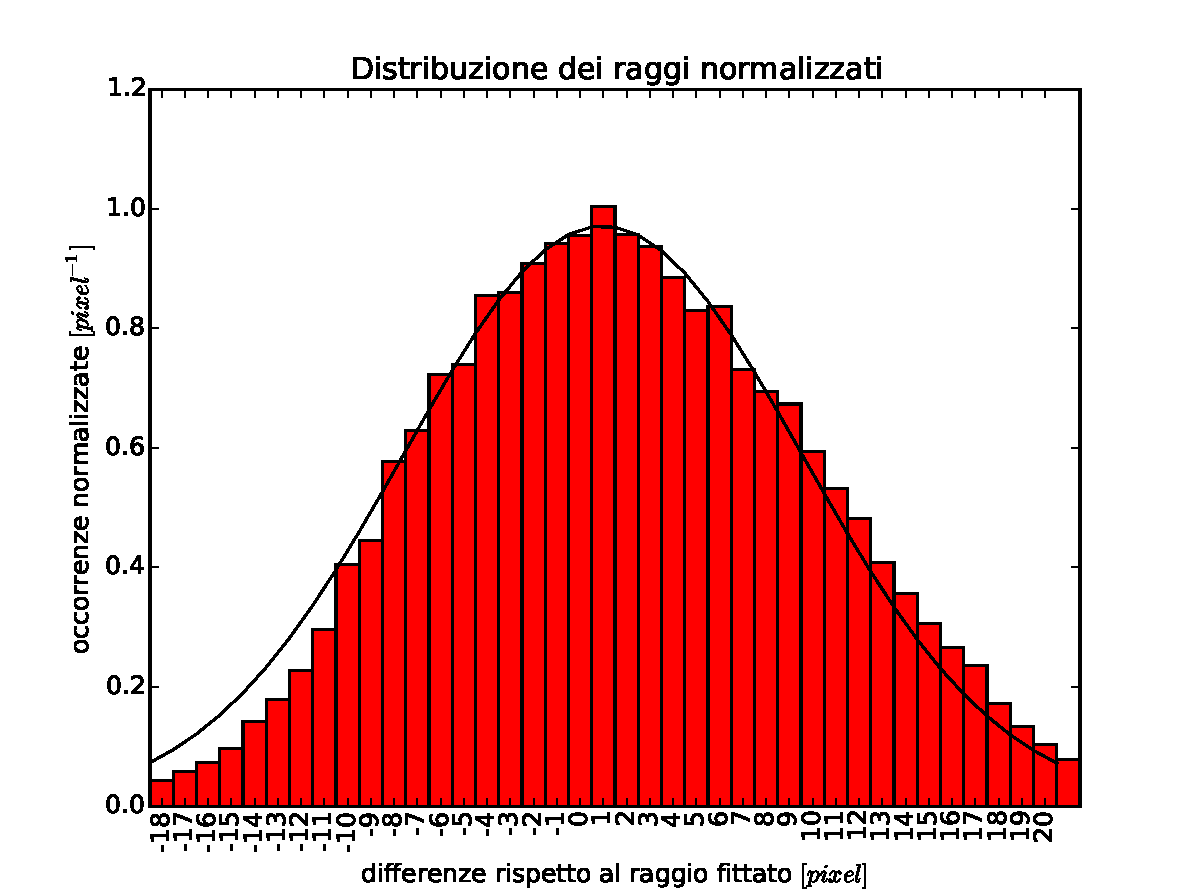
\includegraphics[scale=0.42]{fit_9.pdf}}
	\subfloat{
		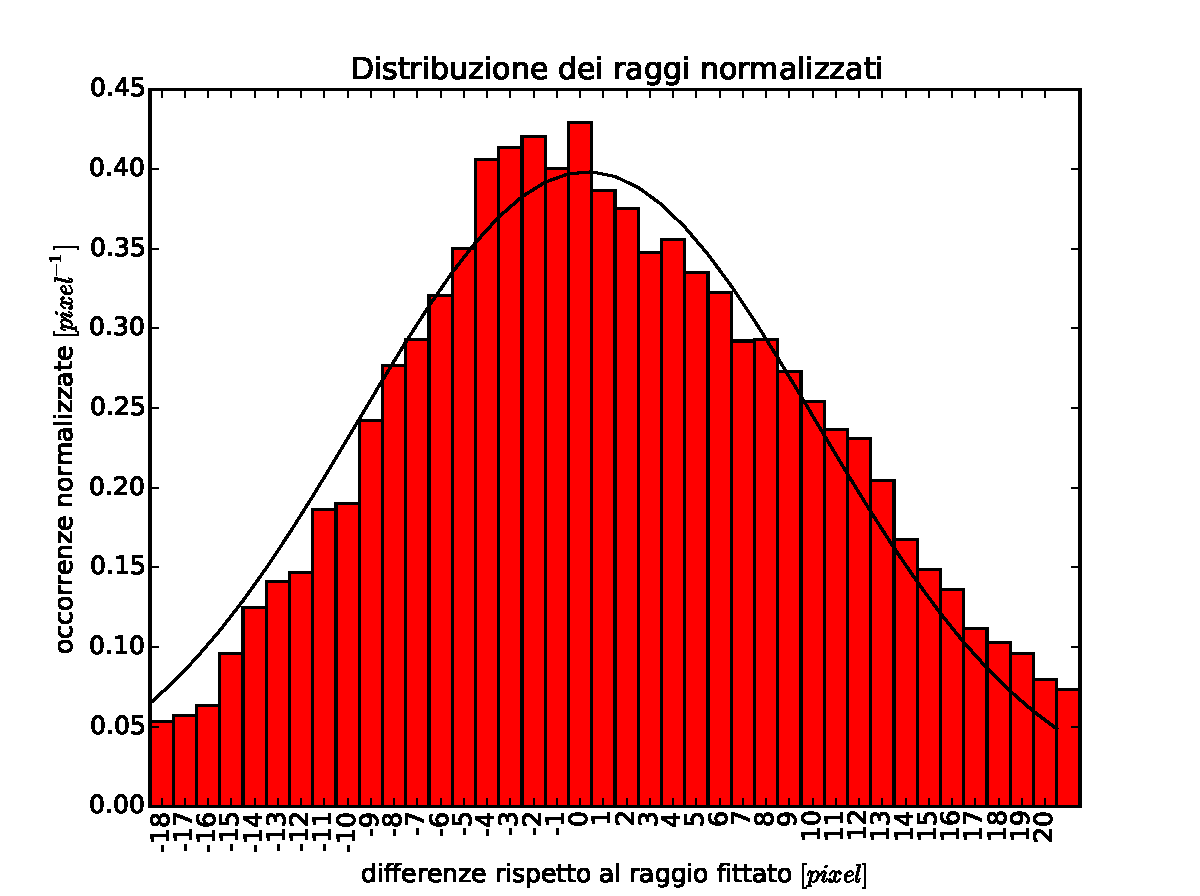
\includegraphics[scale=0.42]{fit_10.pdf}}
	\caption{stima dell'errore sulla misura dei raggi}
	\label{gauss}
\end{figure}

\subsection{Misura del fattore di conversione px/m}

Ottenuta la misura dei raggi e le relative incertezze è necessario convertire la misura da pixel a metri, per farlo si è acquisita una foto del righello nell'apparato, senza il bulbo, come visibile in \figurename{ \ref{righello}}. Si è misurata la distanza tra i due estremi (per minimizzare l'errore sul posizionamento del centro della tacca) e si è preso come errore l'estensione in pixel della tacca sul righello.

Il fattore di conversione così determinato è di $k = \SI{181.9(3)}{px/\cm}$.

Questa prima stima va corretta per per l'effetto della prospettiva (il righello si trova dietro al piano dell'orbita degli elettroni) e per gli effetti di distorsione ottica del bulbo.

\begin{figure}[H]
	\centering
	\includegraphics[scale=0.3]{NO.JPG}
	\caption{foto della scala graduata di calibrazione}
	\label{righello}
\end{figure}

\paragraph{Prospettiva}	Si è misurata la distanza dell'obiettivo della macchina fotografica dal righello e la distanza di questo dal centro del bulbo. Anche se la risoluzione del metro è \SI{1}{\mm} si è valutato di non avere tale precisione nella determinazione del centro del bulbo e nel posizionamento del metro, la misura è stata perciò ripetuta da ogni membro del gruppo e si è preso l'errore massimo. 
% è falso ma è guisto per non dire che il nuovo errore è a caso

I risultati delle misure sono $d_{OR} = \SI{56.5 \pm 0.3}{\cm}$ (distanza obiettivo/righello) e $d_{RB} = \SI{11 \pm 0.2}{\cm}$ (distanza righello/bulbo).
Il fattore di correzione alla misura precedente è di $c = {1.242 \pm 0.003}$, da cui si ottiene una fattore di conversione corretto di $k_c = \SI{225.9 \pm 0.6}{px/\cm}$.

\paragraph{Distorsione del bulbo} Non è banale determinare l'entità della distorsione alla forma delle tracce dovuta alla presenza del bulbo di vetro.

L'osservazione della distorsione prodotta sulla scala graduata del righello non ci da molte informazioni poiché la scala graduata si trova dietro al bulbo e per arrivare all'obiettivo passa due volte per il vetro e l'effetto del primo passaggio è opposto a quello del secondo. La visibile distorsione della scala graduata è dovuta al fatto che dopo il primo passaggio, i raggi proseguono  nel bulbo deviati e urtano la seconda faccia ad un angolo diverso, per cui l'effetto della seconda faccia non è esattamente opposto a quello della prima.

Tuttavia questo effetto è diverso da quello subito dagli oggetti all'interno del bulbo che attraversano una sola faccia e a priori non è detto che abbia lo stesso ordine di grandezza.

Usando l'ottica geometrica una prima approssimazione potrebbe essere quella di considerare localmente il bulbo come un lastra di vetro piatta nel punto di intersezione dei raggi luminosi, come illustrato in \figurename{ \ref{ottica1}}.

\begin{figure}[H]
	\centering
	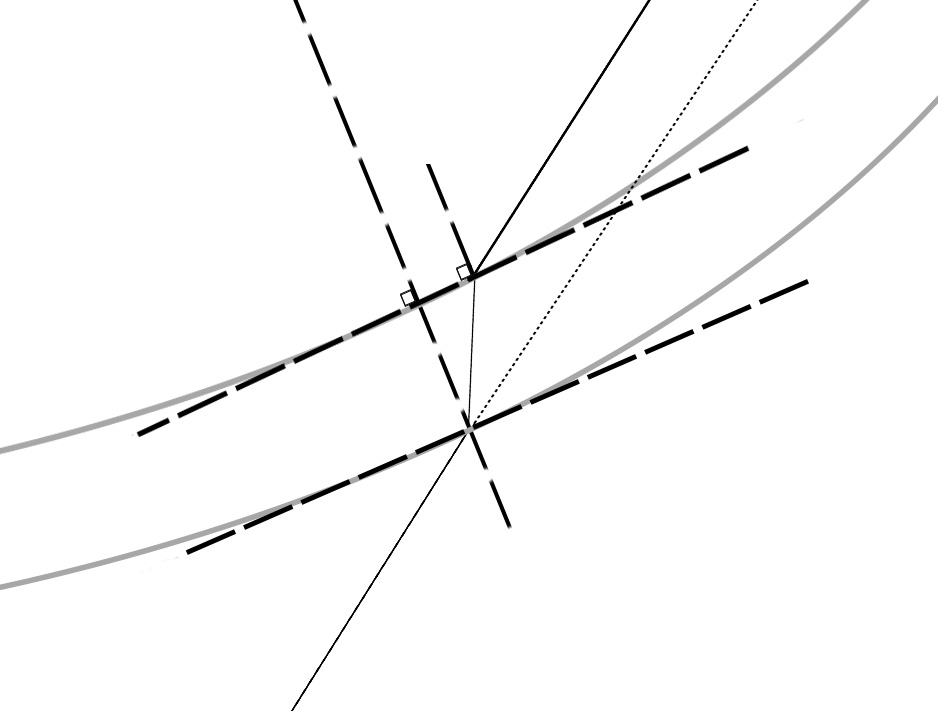
\includegraphics[scale=1]{prima_approx.JPG}
	\caption{schema dei raggi luminosi passanti per il bulbo}
	\label{ottica1}
\end{figure}

I raggi luminosi provenienti dalle tracce (in alto in \figurename{ \ref{ottica1}}) intersecano la superficie interna del bulbo ad una certa inclinazione, proseguono nel vetro con un angolo più piccolo rispetto alla perpendicolare, quindi intersecano la superficie esterna. In questa approssimazione l'angolo di uscita sarà lo stesso di quello di entrata.

Il risultato è che il punto all'interno del bulbo sembrerà più esterno, tuttavia lo spostamento è nel peggiore dei casi pari allo spessore del vetro, che ragionevolmente non sarà più grande di $1-2 \;\text{mm}$. Rispetto ai raggi tipici misurati ($\sim \SI{5}{\cm}$) si tratterebbe di una correzione dell'ordine del $\sim 2-4\%$, quindi a priori non trascurabile.

In realtà questa non è una buona approssimazione sul bordo (dove misuriamo buona parte delle nostre tracce), come visibile in \figurename{ \ref{ottica2}}.

\begin{figure}[H]
	\centering
	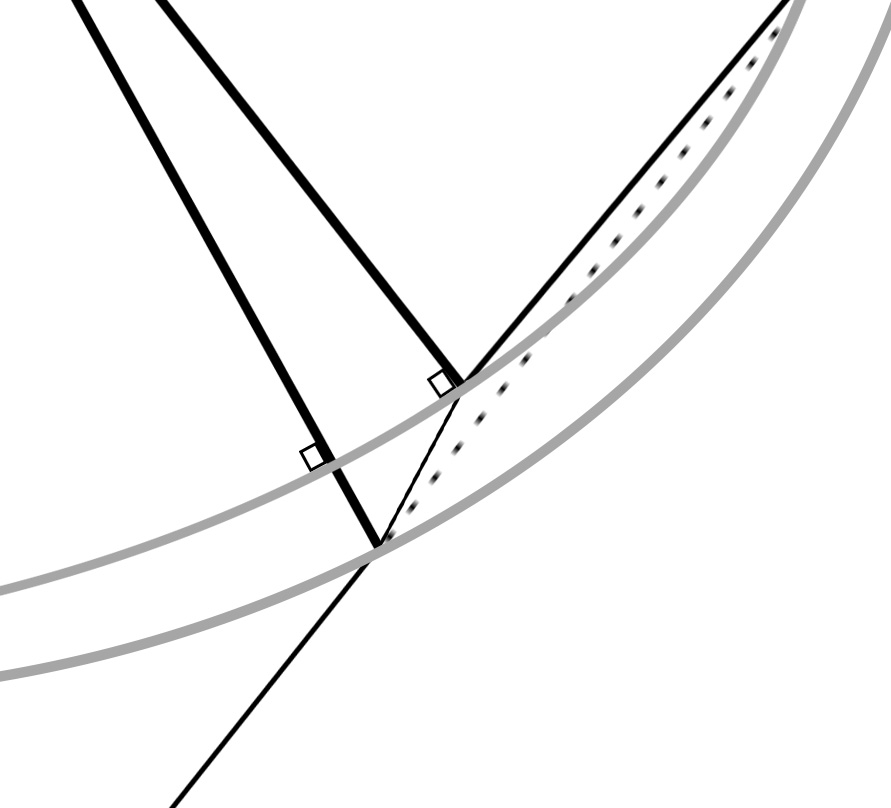
\includegraphics[scale=0.8]{seconda_approx.JPG}
	\caption{schema dei raggi luminosi passanti per il bulbo}
	\label{ottica2}
\end{figure}

Come prima i raggi luminosi provenienti dalle tracce (in alto in \figurename{ \ref{ottica2}}) intersecano la superficie interna ad un certo angolo e proseguono nel vetro come nel caso precedente. Tuttavia la seconda intersezione avviene ad un angolo diverso dal precedente e l'angolo di uscita (rispetto alla perpendicolare) sarà minore.

Il risultato è che in base alla posizione del punto nel bulbo questo potrebbe sembrare più interno. Questo effetto opposto a quello visto sopra potrebbe a priori avere lo stesso ordine di grandezza.

Si è proceduto con l'ottica geometrica al calcolo della funzione che dato il raggio misurato ci dia il raggio corretto e si riporta in \figurename{ \ref{bulbo}} il grafico del fattore di correzione . Nel calcolo si è stimato il raggio del bulbo $R \sim \SI{6.4}{\cm}$ (misurato a partire dalle foto, noto il fattore di conversione prima calcolato), l'indice di rifrazione $n \sim 1.6$ (un vetro generico) e lo spessore di $d \sim \SI{1}{\mm}$.

La correzione finale è quindi dell'ordine del $2-3\%$ e solo per raggi maggiori di \SI{6}{\cm}.

\begin{figure}[H]
	\centering
	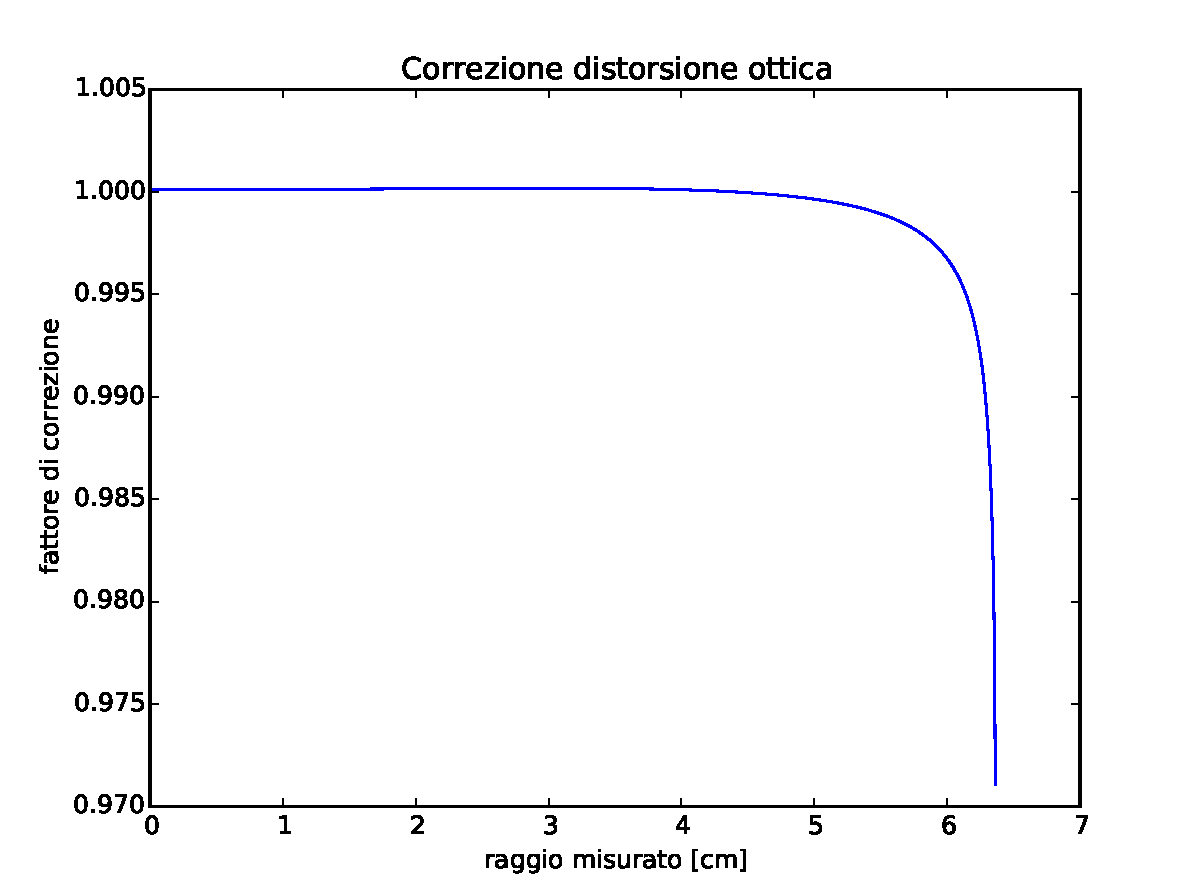
\includegraphics[scale=0.7]{bulbo.pdf}
	\caption{Correzione al fattore di conversione}
	\label{bulbo}
\end{figure}

Nella conversione dei raggi in metri abbiamo tenuto conto di questa correzione facendo quindi l'approssimazione che le circonferenze abbiano centro nel centro del bulbo.
I dati relativi a tutte le acquisizione effettuate, i raggi fittati e i relativi errori sono riportati in appendice in \tablename{ \ref{dati_raggi}}.

\section{Misura di $V$}
La misura di $V$ è fatta dal generatore di tensione del cannone elettronico ed è nota con una risoluzione di \SI{1}{\volt} che si è assunto come errore (andrebbe aggiunto l'errore di calibrazione che è ignoto).

La misura di $V$ è correlata alla determinazione della velocità degli elettroni in uscita dal cannone elettronico e come fatto notare nel datasheet dell'apparato la più grande sorgente di errore nell'esperimento è la non uniformità del campo accelerante, causato dal buco nell'anodo che porta la velocità degli elettroni ad essere inferiore a quella attesa, per cui la misura di $\tfrac{e}{m}$ sarà fortemente affetta da questo effetto.

Non è possibile tenere conto di questi effetti a meno di conoscere esattamente la geometria del cannone elettronico, sappiamo comunque che l'effetto sarà quello di aumentare il valore di  $\tfrac{e}{m}$ sperimentale rispetto a quello teorico.

\section{Calcolo di e/m}
A partire dalle misure effettuate si è proceduto al calcolo di $\tfrac{e}{m}$, si sono quindi mediate le misure a pari $V$ e, tenuto conto di tutte le correzioni esposte nei punti precedenti, i risultati sono i seguenti:

\begin{table}[H]
	\centering
	\begin{tabular}{ccc}
		\toprule
		$V$ [\si{\volt}] & 	$\frac{e}{m}$ [C/Kg] \\
		\midrule
$	200 \pm 1	$ & $	2.76 \pm 0.08	$ \\
$	219 \pm 1	$ & $	2.81 \pm 0.08	$ \\
$	232 \pm 1	$ & $	2.83 \pm 0.09	$ \\
$	261 \pm 1	$ & $	2.92 \pm 0.10	$ \\
$	282 \pm 1	$ & $	2.97 \pm 0.10	$ \\
$	302 \pm 1	$ & $	2.97 \pm 0.13	$ \\
\bottomrule
\end{tabular}
\end{table}

\section{Conclusioni}
Come è chiaro i risultati sono assolutamente incompatibili con il valore noto di $\SI{1.76}{C/Kg}$.

Tuttavia questo risultato era atteso: il datasheet dell'apparato riporta che con questa strumentazione, dato l'errore sulla velocità, il risultato della misura di $\tfrac{e}{m}$ eccederà il valore noto di $\sim \SI{1.1}{C/Kg}$.
È possibile confrontare il grafico presente nel datasheet riportato in \figurename{ \ref{grafico_farlocco}} con i risulti delle nostre misure in \figurename{ \ref{dati_nostri}} e notare che i valori trovati sono compatibili.

\begin{figure}[H]
	\centering
	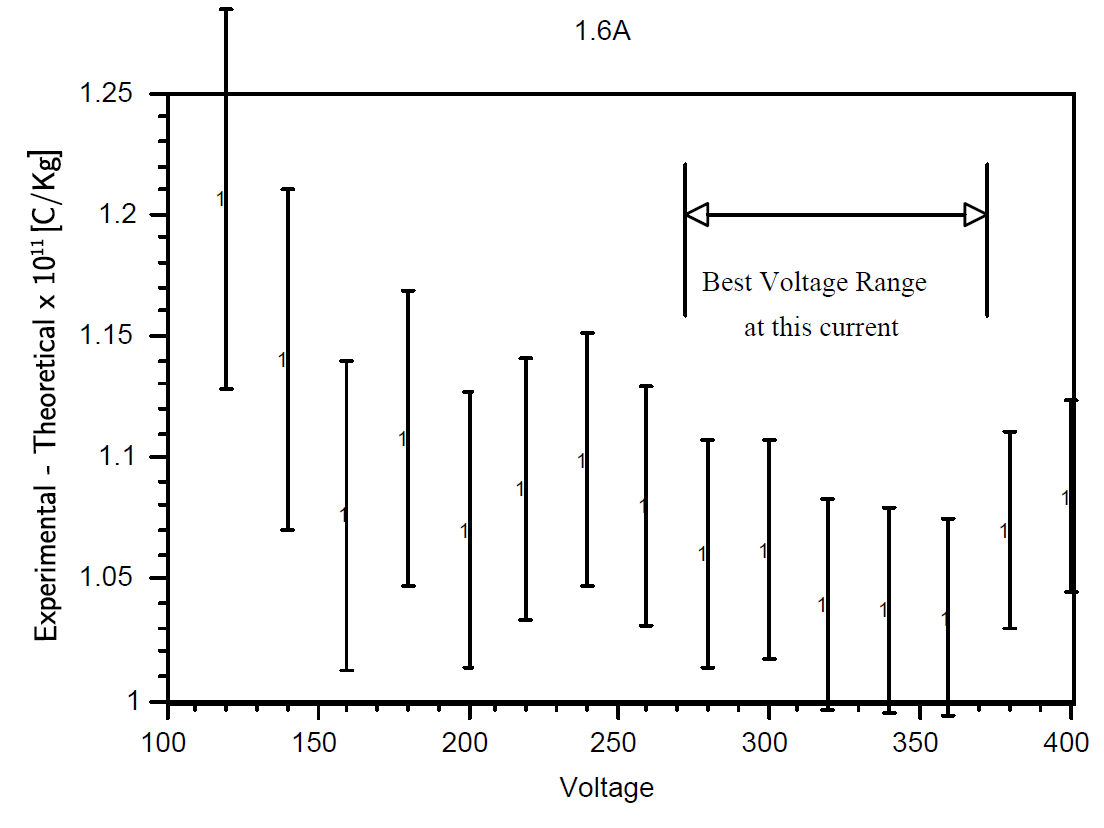
\includegraphics[scale=0.3]{farlocco.png}6
	\caption{Grafico riportato nel datasheet dell'apparato}
	\label{grafico_farlocco}
\end{figure}

\begin{figure}[H]
	\centering
	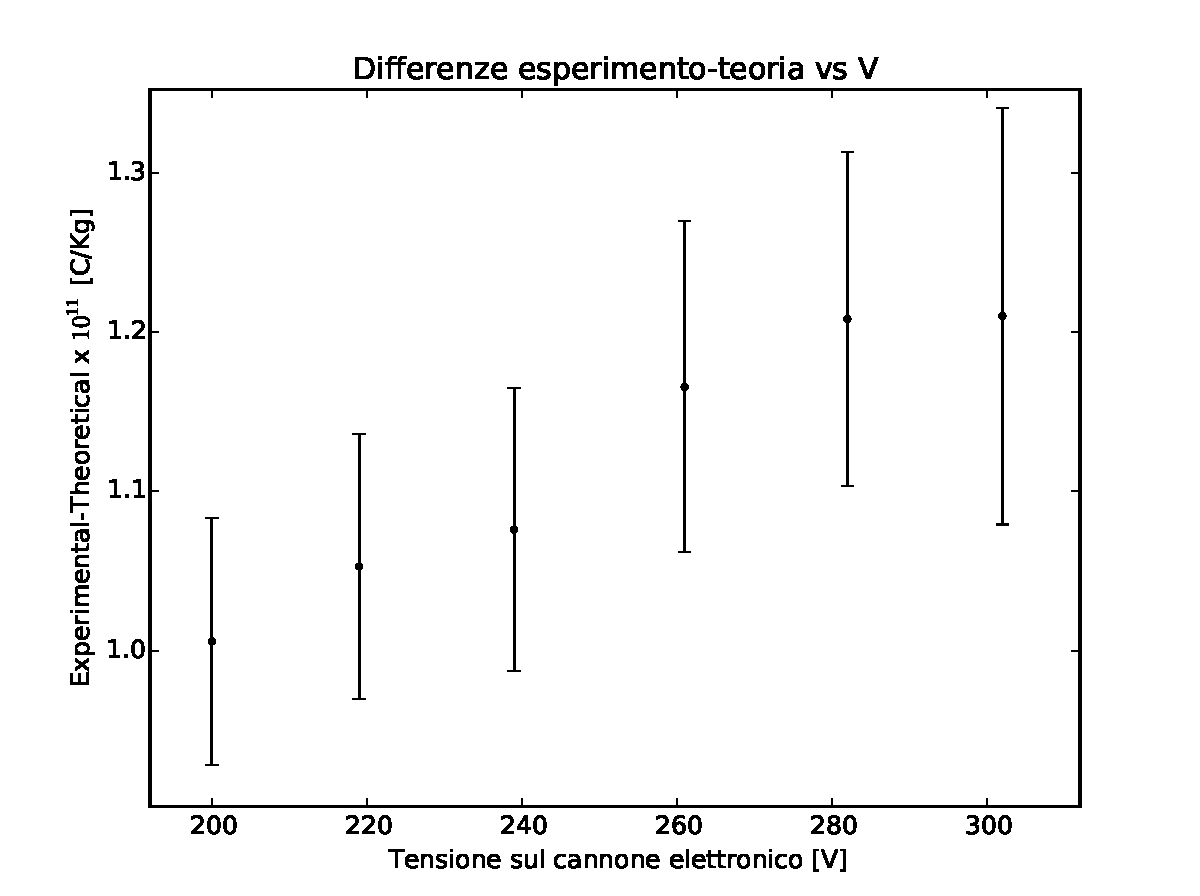
\includegraphics[scale=0.62]{dm.pdf}
	\caption{Confronto esperimento/teoria con i nostri dati}
	\label{dati_nostri}
\end{figure}


\newpage
\section{Appendice}

	\begin{table}[h]
		\centering
		\begin{tabular}{ccccc}
			\toprule
			$l$ [\si{cm}]	& 	$V_{out}$ [\si{\volt}]	&& 	$l$ [\si{cm}]	& 	$V_{out}$ [\si{\volt}] \\
			\midrule
			14.0 	& 	 0.405	&&	25.5	& 	 0.407 \\
			14.5	& 	 0.407	&&	20.5	& 	 0.410 \\
			15.0	& 	 0.408	&&	21.0	& 	 0.410 \\
			15.5	& 	 0.408	&&	21.5	& 	 0.409 \\
			16.0	& 	 0.408	&&	22.0	& 	 0.410 \\
			16.5	& 	 0.409	&&	22.5	& 	 0.410 \\
			17.0	& 	 0.409	&&	23.0	& 	 0.410 \\
			17.5	& 	 0.409	&&	23.5	& 	 0.409 \\
			18.0	& 	 0.409	&&	24.0	& 	 0.409 \\
			18.5	& 	 0.409	&&	24.5	& 	 0.409 \\
			19.0	& 	 0.409	&&	25.0	& 	 0.408 \\
			19.5	& 	 0.409	&&	25.0	& 	 0.408 \\
			20.0	& 	 0.409	&&	26.0	& 	 0.406 \\
			\bottomrule
		\end{tabular}
		\caption{Mappatura del campo magnetico all'interno della bobina di Helmholtz.}
		\label{tab:a}
	\end{table}

\begin{table}[hb]
\centering
\begin{tabular}{ccc}
	\toprule
$V$ [\si{\volt}] & 	$I$ [\si{\ampere}] & $r$ [\si{\cm}]\\
\midrule
$200	\pm 1 $	 	&	$0.99 \pm 0.01 $	&	$1104 \pm 	11$	\\
$200	\pm 1 $		&	$1.03 \pm 0.01 $	&	$1077 \pm 	10$	\\
$200	\pm 1 $		&	$1.07 \pm 0.01 $	&	$1041 \pm 	9$	\\
$200	\pm 1 $		&	$1.10 \pm 0.01 $	&	$1015 \pm 	10$	\\
$200	\pm 1 $		&	$1.15 \pm 0.01 $	&	$935 \pm  	11$	\\
$219	\pm 1 $		&	$1.03 \pm 0.01 $	&	$1108 \pm 	16$	\\
$219	\pm 1 $		&	$1.07 \pm 0.01 $	&	$1097 \pm 	13$	\\
$219	\pm 1 $		&	$1.10 \pm 0.01 $	&	$1056 \pm 	16$	\\
$219	\pm 1 $		&	$1.15 \pm 0.01 $	&	$1044 \pm 	16$	\\
$239	\pm 1 $		&	$1.07 \pm 0.01 $	&	$1099 \pm 	18$	\\
$239	\pm 1 $		&	$1.15 \pm 0.01 $	&	$1075 \pm 	17$	\\
$261	\pm 1 $		&	$1.07 \pm 0.01 $	&	$1110 \pm 	18$	\\
$261	\pm 1 $		&	$1.10 \pm 0.01 $	&	$1109 \pm 	17$	\\
$261	\pm 1 $		&	$1.14 \pm 0.01 $	&	$1091 \pm 	16$	\\
$282	\pm 1 $		&	$1.07 \pm 0.01 $	&	$1199 \pm 	16$	\\
$282	\pm 1 $		&	$1.10 \pm 0.01 $	&	$1124 \pm 	20$	\\
$282	\pm 1 $		&	$1.15 \pm 0.01 $	&	$1106 \pm 	20$	\\
$302	\pm 1 $		&	$1.10 \pm 0.01 $	&	$1193 \pm 	19$	\\
$302	\pm 1 $		&	$1.15 \pm 0.01 $	&	$1123 \pm 	21$	\\
\bottomrule
\end{tabular}
\caption{Dati di tutte le acquisizioni}
\label{dati_raggi}
\end{table}

	
	
	
	
	
	
	
	
	
	
	
	
	
	
	
	
	
	
	
	
	
	
\end{document}
